%Analýza a návrh řešení konkrétního problému

%Analýza a návrh řešení problému z oblasti úzce související se 
%softwarovým či datovým inženýrstvím nebo systémovým prostředím.
%Výsledkem je výzkumná zpráva a prototypové řešení.



%Vypracování musí demonstrovat pochopení problému. Tedy práce by
%neměla pouze slepě následovat první zjevnou cestu k řešení, či
%cestu naznačenou v zadání. Autor musí ze všeho nejdříve ukázat, že
%chápe, jaký problém má řešit, a že je schopen vysvětlit, čeho a
%proč chce dosáhnout.

%Text práce má dokumentovat postup vypracování řešení tak, aby bylo
%možné posoudit, zda si autor počínal vhodně, a zda si byl vědom
%souvislostí, které jeho vypracování ovlivňují. Tedy je třeba
%systematicky a přehledně vysvětlit a zdůvodnit důležitá rozhodnutí
%učiněná při vypracování práce. Text práce má popisovat zvolené
%řešení strukturovaně shora dolů, a zabíhat do detailu pouze v
%případech nestandardních postupů nebo rozhodnutí.

%Pokud práce z prostorových či kapacitních důvodů neobsahuje
%nejlepší možné řešení problému, měla by vysvětlit, jak by
%optimální řešení mohlo vypadat.

%Hrubá osnova výzkumné zprávy:

%1.         Úvod charakterizující kontext problému - introduction
%2.         Přesné vymezení problému 
%3.         Přesné vymezení cílů návrhu
%4.         Struktura práce ve vztahu k vytyčeným cílům
%5.         Analýza problému z různých hledisek
%6.         Návrh řešení s diskusí alternativ
%7.         Rozpracování vybraného přístupu
%8.         Popis prototypové implementace
%9.         Zhodnocení splnění cílů a srovnání s jinými známými přístupy
%10.        Závěr se stručným shrnutím výsledků a přínosu
%11.        Seznam citované literatury

%Implementace musí být odevzdána jednak v podobě zdrojových souborů a všech dat potřebných k jejímu překladu a spuštění, jednak v již přeložené a spustitelné podobě. Na zdrojových souborech musí být jasně patrné, které části implementace jsou autorovým původním dílem, a které jsou převzaté (generovaný kód, knihovny ...).

%Spustitelná podoba práce musí demonstrovat funkčnost implementace. Pokud je k takové demonstraci potřeba netriviální prostředí či nastavení, autor práce jí musí na požádání předvést vedoucímu a oponentovi, případně také hodnotící komisi.

%Branova varianta: 
\documentclass[a4paper,12pt]{report}
\usepackage[height=29.7cm, width=21cm, left=3cm, right=2cm, top=3cm, bottom=2cm, includefoot]{geometry}

\usepackage[utf8]{inputenc}
%\documentclass [10pt]{report}

\title{The Tool for Modeling of Evolution of the Artificial Life}
\author{Iva Bartů\v{n}kov\'{a}}

\usepackage{url}
\usepackage{graphicx} %mohla bych pridat [driver] coze je ze to chci bud do ps nebo do pdf.
%\usepackage{listings}

\begin{document}

%%%%%%%%%%%%%%%%%%%%%%%%%%% Titulni stranka %%%%%%%%%%%%%%%%%%%%%%%%
\begin{titlepage}
\begin{center}
\vspace{15mm}
\large
Univerzita Karlova v Praze\\
Matematicko-fyzikální fakulta\\

\vspace{5mm}

{\Large\bf DIPLOMOV\'{A} PR\'{A}CE}

\vspace{10mm}

% MFF LOGO

\begin{center}
  \includegraphics[scale=0.7]{images/logo.eps}
\end{center}


\vspace{15mm}

%\normalsize
{\Large Iva Bartů\v{n}kov\'{a}}\\
\vspace{5mm}
{\Large\bf N\'{a}stroj pro modelov\'{a}n\'{i} evoluce um\v{e}l\'{e}ho \v{z}ivota} \\
{\Large\bf The Tool for Modeling of Evolution of the Artificial Life} \\
\vspace{5mm}
Kabinet software a v\'{y}uky informatiky



\vspace{15mm}
\large
\noindent Vedoucí diplomové práce: RNDr. Tom\'{a}\v{s} Holan, Ph.D.
\vspace{1mm} 

\noindent Studijní program: Informatika, architektura a principy softwarov\'{y}ch syst\'{e}mů %doplňte odpovídající údaje

\vspace{20mm}

2007
\end{center}

\end{titlepage}
%%%%%%%%%%%%%%%%%%%%%%%%%%%%%%%%%%%%%%%%%%%%%%%%%%%%%%%%%%%%%%%%%%%%%%%%%%%%%%
\normalsize % nastavení normální velikosti fontu
\setcounter{page}{2} % nastavení číslování stránek
\ \vspace{10mm} 

\noindent 
%Na tomto místě mohou být napsána případná poděkování (vedoucímu práce, konzultantovi, tomu, kdo půjčil software, 
%literaturu, poskytl data apod.). % doplňte vlastní text

%We thank to DIMACS at Rutgers University for supporting this research 
%during REU. Many helpful comments and ideas by Ji\v{r}\'{i} Fiala and 
%Martin Tancer improved the whole work. This should be in Czech.

Děkuji RNDr. Tomášovi Holanovi, Ph.D. za vedení práce a inspiraci, Jiřímu Svobodovi a RNDr. Františku Mrázovi, CSc. za konzultace k návrhu řešení. 

\vspace{\fill} % nastavuje dynamické umístění následujícího textu do spodní části stránky
\noindent Prohlašuji, že jsem svou diplomovou práci napsala samostatně a výhradně s použitím citovaných pramenů. Souhlasím se zapůjčováním práce a jejím zveřejňováním.

\bigskip
\noindent V Praze dne \hspace{\fill}Iva Bartů\v{n}kov\'{a}\\ % doplňte patřičné datum, jméno a příjmení

%%%   Výtisk pak na tomto míste nezapomeňte PODEPSAT!
%%%                                         *********
%%%%%%%%%%%%%%%%%%%%%%%%%%%%%  Obsah

\tableofcontents % vkládá automaticky generovaný obsah dokumentu


%%%%%%%%%%%%%%%%%%%%%%%%%%%%%  Page with abstracts

\newpage % přechod na novou stránku
%%%%%%%%%%%%%%%%%%%%%%%%%%%%%  Page with abstracts

\newpage % přechod na novou stránku

\noindent
Název práce: N\'{a}stroj pro modelov\'{a}n\'{i} evoluce um\v{e}l\'{e}ho \v{z}ivota\\
Autor: Iva Bartů\v{n}kov\'{a}\\
Katedra (ústav): Kabinet software a v\'{y}uky informatiky\\
Vedoucí diplomové práce: RNDr. Tom\'{a}\v{s} Holan, Ph.D.\\
e-mail vedoucího: Tomas.Holan@mff.cuni.cz\\

\noindent Abstrakt: V práci studujeme problematiku simulátorů modelujících umělý život. Práce navrhuje a předkládá softwarový nástroj, umožňující provádět experimenty s vývojem jednoduchých organismů, jejichž genom je tvořen sadou parametrů. Popisuje provedené experimenty a dosažené výsledky.


%V předložené práci studujeme seznamové barvení rovinných grafů. Seznamové barvení je varianta problému barvení grafu, kde každý vrchol má přidělený svůj vlastní seznam možných barev. Říkáme, že graf je $k$-vybíravý, je-li možné nalézt dobré obarvení pokaždé, když všechny seznamy obsahují alespoň $k$ barev. 

%Je známo, že každý rovinný graf bez trojúhelníků je 4-vybíravý a každý rovinný bipartitní graf (t.j. bez lichých cyklů) je 3-vybíravý. Práce ukazuje postačující podmínky pro 3-vybíravost rovinných grafů bez troj\-úhel\-níků s omezeným výskytem krátkých cyklů.

%Dále práce ukazuje konstrukci rovinného grafu bez
%trojúhelníků který není 3-vybíravý a to na menším počtu
%vrcholů, než potřebují doposud známé konstrukce.

\vspace{8mm}

\noindent Klíčová slova: umělý život, evoluce, simulátor

\vspace{10mm}

\noindent
Title: The Tool for Modeling of Evolution of the Artificial Life\\
Author: Iva Bartů\v{n}kov\'{a}\\
Department: Department of Software and Computer Science Education\\
Supervisor: RNDr. Tom\'{a}\v{s} Holan, Ph.D.\\
Supervisor's e-mail address: Tomas.Holan@mff.cuni.cz\\

\noindent Abstract: In the thesis we concern with simulators of artificial life. The thesis models and submits a software simulator for research on evolution of simple organisms. Conducted experiments and their results are described. 
 
\vspace{8mm}

\noindent Keywords: artificial life, evolution, simulator


%\begin{abstract}
%Target of thesis is to create a software simulator allowing experiments with the evolution of simple organisms, run several experiments and describe results.
%\end{abstract}


\chapter{Introduction to Artificial Life}

%*************3 pages about 1.Artificial life - definition, history, contemporary course 2. Brief context of my thesis*******************************

%******************Definition of Artificial life*********************
\section{What is Artificial Life?}
Artificial Life, (commonly \textbf{Alife} or \textbf{alife}) is a field of study and an art form that examines systems related to life, its processes and its evolution through simulations using computer models, robotics, and biochemistry (called "soft", "hard", and "wet" approaches respectively \cite{Bedau}).

In this thesis the term "Artificial Life" is often used to specifically refer to soft alife.

The term Artificial life was first coined by Christopher Langton in the late 1980s at the first "International Conference on the Synthesis and Simulation of Living Systems" (otherwise known as Artificial Life I) at the Los Alamos National Laboratory in 1987. He envisioned a study of life as it could be in any possible setting.

Artificial life studies "natural" life by attempting to recreate biological phenomena from scratch within non-living media like computers or RNA structures of molecules. Alife complements the traditional analytic approach of traditional biology with a synthetic approach in which, rather than studying biological phenomena by taking apart living organisms to see how they work, one attempts to put together systems that behave like living organisms.

The process of synthesis has been an extremely important tool in many disciplines. Synthetic chemistry --- the ability to put together new chemical compounds not found in nature --- has not only contributed enormously to our theoretical understanding of chemical phenomena, but has also allowed us to fabricate new materials and chemicals that are of great practical use for industry and technology.

Artificial life amounts to the practice of "synthetic biology" and, by analogy with synthetic chemistry, the attempt to recreate biological phenomena in alternative media will result in not only better theoretical understanding of the phenomena under study, but also in practical applications of biological principles in the technology of computer hardware and software.\cite{Langton} 

The seminal novelty of ALife lies in its synthetic approach. Whereas traditional research is essentially analytic, breaking down complex systems into basic components, Alife attempts to construct complex systems from elemental units.\cite{BornhoffenLataud}

For example, answering of questions like how the simple rules of Darwinian evolution lead to high-level structure, or the way in which the simple interactions between ants and their environment lead to complex trail-following behavior promises to provide novel solutions to complex real-world problems, such as disease prevention, stock-market prediction, and data-mining on the Internet.\cite{AdamiBrown}

%************History of Alife as a science
%The only source: Wikipedia - History of artificial life. However, citations are poor in this article. 
%Exists:Artificial Life and the Sciences of Complexity: History and Future, 	Jean-Claude Heudin. But it is not accessible for free.
%1hour of searching. Lets stop it.
\section{History of Artificial Life}

Important events at development of mathematics and computer science that later led to ideas of artificial life were presented in late 1940s at the Hixon Symposium in California. Math and computer prodigy John Von Neumann delivered a lecture titled "The General and Logical Theory of Automata" where he defined the term "automaton" and said that natural organisms would in the end be found to follow similar simple rules. He postulated a machine, "kinematic automaton", that could create an identical machine. Later he crated one with Stanislaw Ulam, a purely logic-based automata, not requiring a physical body but based on the changing states of the cells in an infinite grid --- the first cellular automaton (CA). It was extraordinarily complicated compared to later CAs, having hundreds of thousands of cells which could each exist in one of twenty-nine states.
 
Celular automata were first field of artificial life in computer science and they are important up to present. A cellular automaton is a discrete model that consists of a regular grid of cells, each in one of a finite number of states. The grid can be in any finite number of dimensions. Time is also discrete, and the state of a cell at time t is a function of the states of a finite number of cells (called its neighborhood) at time $t - 1$. These neighbors are a selection of cells relative to the specified cell, and do not change. Every cell has the same rule for updating, based on the values in this neighbourhood. Each time the rules are applied to the whole grid a new generation is created.\cite{Delorme} 

The following important step towards Artificial life was realized by Edgar F. Codd, who simplified Von Neumann's original twenty-nine state monster to one with only eight states.
 
The history of Artificial life dates back to 1987 when the "International Conference on the Synthesis and Simulation of Living Systems" (otherwise known as Artificial Life I) was held at the Los Alamos National Laboratory. Researcher Christopher Langton defined here his idea of new science that had barely existed up to that time.
 
In 1977 founded Ed Fredkin the Information Mechanics Group at MIT, \url{http://www.ai.mit.edu/projects/im/}. This group created a computer especially designed to execute cellular automata, eventually reducing it to the size of a single circuit board. This "cellular automata machine" allowed an explosion of alife research among scientists who could not otherwise afford sophisticated computers.

In 1982, computer scientist Stephen Wolfram turned his attention to cellular automata. He explored and categorized the types of complexity displayed by one-dimensional CAs, and showed how they applied to natural phenomena such as the patterns of seashells and the nature of plant growth. 

Computer animator Craig Reynolds similarly used three simple rules to create recognizable flocking behavior in groups of computer-drawn "boids" in 1987. With no top-down programming at all, the boids produced life-like solutions to evading obstacles placed in their path. Computer animation has continued to be a key commercial driver of alife research as the creators of movies attempt to find more realistic and inexpensive ways to animate natural forms such as plant life, animal movement, hair growth, and complicated organic textures.

The Unit of Theoretical Behavioral Ecology at the Free University of Brussels applied the self-organization theories to model behavior of swarms and colonies of organisms.

A conference in May of 1985 called "Evolution, Games, and Learning" focused Alife to tie to the emerging field of complex adaptive systems. Key figure was J. Doyne Farmer working at the Center for Nonlinear Studies.

In 2000s the field is underway to create cellular models of artificial life. Initial work on building a complete biochemical model of cellular behavior is underway as part of a number of different research projects, namely BlueGene which seeks to understand the mechanisms behind protein folding.

The current progress in Artificial life is regularly presented at Alife ---International Conference on the Simulation and Synthesis of Living Systems and ECAL ---- European Conference on Artificial Life organized by International Society of Artificial Life (ISAL), \url{http://www.alife.org}. 

\section{Abeetles --- Simulator of Artificial life}

%***********This thesis is about -> software, target of this work: 1.set of features 2.simulator 3.experiments
This thesis is bounded within software approach to Artificial life. Its main target is to design and create software simulator Abeetles. Abeetles runs life of simple organisms in its specific environment and is concerned with evolution of their features and behavior. The system avails experiments with evolution of the organisms under various conditions and offer overviews and statistics of the process. Experiments performed with the system will be described in chapter Experiments.

%This is here out of context.
%Artificial life can be split into various subfields according to chosen substrat of the system (digital, mechanical or test-tube) as well as according to aspect of natural life, that is in the focus of the research.


%replace this to another chapter!!
%*************Evolutionary computation: if we choose evolution of biological life as the topic of our artificial life exploration and simulate it using computers.
%One of terms related to Artificial life is Evolutionary computation. It is a general term for several computational techniques which are based to some degree on the evolution of biological life in the natural world and simulated using computers. Evolutionary computation thus uses techniques of natural world and applies them using computers in other fields of interest. The most widely used form of evolutionary computation are Genetic Algorithms. Evolution techniques are often focused on evolution of moving, shape, visual art and music. 



\section{Related Terms}
Abeetles concerns with evolution and genetics. They originate from biology and therefore their definition is also biological. Following terms will be used in this thesis: gene, genome, genotype and phenotype.

Gene is a structural unit of inheritance in living organisms. A gene is, in essence, a segment of DNA that has a particular purpose, i.e., that codes for (contains the chemical information necessary for the creation of) a specific enzyme or other protein.\cite{GeneDic}

In biology the genome of an organism is its whole hereditary information and is encoded in the DNA (or, for some viruses, RNA). This includes both the genes and the non-coding sequences of the DNA. The term was coined as a portmanteau of the words gene and chromosome.\cite{GenomeDef}

The genotype of an organism is the class to which that organism belongs as determined by the description of the actual physical material made up of DNA that was passed to the organism by its parents at the organism's conception. For sexually reproducing organisms that physical material consists of the DNA contributed to the fertilized egg by the sperm and egg of its two parents. For asexually reproducing organisms, for example bacteria, the inherited material is a direct copy of the DNA of its parent. 

The phenotype of an organism is the class to which that organism belongs as determined by the description of the physical and behavioral characteristics of the organism, for example its size and shape, its metabolic activities and its pattern of movement.
\cite{GenPhen}

%Furthemore should be explained: genome


%%%%%%%%%%%%%%%%%%%%%%%%%%%%%%%%%%%%%%%%%%%%%%%%%%%%%%%%%%%%%%%%%%%%%%%%%%%%%
%%%%%%%%%%%%%%%%%%%%%%%%%%%%%%%%%%%%%%%%%%%%%%%%%%%%%%%%%%%%%%%%%%%%%%%%%%%%%
\chapter{Abeetles in Context of Alife Simulators} 
%Přesné vymezení problému
%5 pages about precise definition of the problem - description of chosen existing brother programs and comparison and choice of my objectives. I will use the Porovnani.xls 
%******************Context of my thesis - cathegories of Alife simulators and ranking of my work. Short about existing brother programs and programs that inspired me.
The family of software simulators of artificial life is numerous. Therefore to find a position for a new simulator needs some classification. This thesis will expand on three classification possibilities of Alife simulators. First, categorization according to the method of creature definition will be used. Second, simulators will be distinguished with respect to the feature or features of Artificial life, that they simulate. Third, the criterion of purpose of the simulator and target group of users will be used. The fourth section places Abeetles into these classification systems and thereby specifies sphere of Artificial life that will be dealt in this thesis.

\section{Classification by Creature Definition}
In existing systems individual agents are modeled and constructed in many different ways that rank them roughly into following categories:
\begin{itemize}
    \item \textbf{Program Based} --- In program based simulators an individual is represented by a program which substitutes biological DNA and make up the genome of the agents. Language of the program is usually Turing complete. Assembly derivatives are the most common languages used. Tom Ray's Tierra is a famous example of a program based simulator.
    \item \textbf{Module Based} --- An agent in a module based system is a composition of individual modules. These modules modify the creature's behavior and characteristics either directly, by hard coding into the simulation (leg type A increases speed and metabolism), or indirectly, through the emergent interactions between a creature's modules (leg type A moves up and down with a frequency of X, which interacts with other legs to create motion). Generally these are simulators which emphasize user creation and accessibility over mutation and evolution.  
    \item \textbf{Parameter Based} --- If an organism is constructed to have defined and fixed behavior that is controlled by various parameters that mutate, the system is referred as a parameter based. It means that each organism contains a collection of numbers or other finite parameters. Each parameter controls one or several aspects of the organism in a well defined way.
    \item \textbf{Neural Network Based} --- These systems simulates processes of  creatures that learn and grow using neural networks or a close derivative. Emphasis is often, although not always, more on learning than on natural selection.
\end{itemize}

\section{Classification by Simulated Phenomenon}
Another grouping of simulators can be done according to phenomenon, that they simulate. It is presented at the web page of Monash University’s Complexity Virtual Lab. \url{http://vlab.infotech.monash.edu.au/}
\begin{itemize}
  \item \textbf{Networks} --- Relationships in complex natural systems are simulated according to network theory (or diktyology) as networks or graphs and their statistical and topological properties are analyzed. 
  \item \textbf{Nonlineality} --- Nonlineal systems are systems that cannot be mathematically described as a sum of their components. While certain assumptions can be made for lineal systems, that often make the mathematical modelling of such systems easy, mathematical modelling of nonlineal systems is often very difficult or impossible. As a result, nonlineal systems are often studied through use of simulations.
  \item \textbf{Swarms} --- A swarm is a group of independent agents that gather together in order to collectively carry out a certain task. Typically, each agent exhibits a very simple behavior pattern that is influenced by direct or indirect interactions with other swarm members. As a result, the swarm as a whole may exhibit complex and intelligent behavior patterns. In nature, swarms can be observed in social insects, fish schools, but also in primitive single cell organisms.
  \item \textbf{Evolution} --- Evolution is the process of development or grows by accumulation of small advantageous changes. The study of all forms of evolutionary processes is one of the primary goals of ALife. This includes the study of biological evolution of species as well as other evolutionary processes in natural, artificial and social systems.
  \item \textbf{Cellular Automata} --- The term cellular automaton (CA)is described in the previous chapter. It is not directly a phenomenon of natural life, but it is a discrete model of mutual influence of neighboring elements, which can be in the nature observed. 
\end{itemize}  

\section{Classification by Purpose}
Apparently, the main purpose of Artificial life simulators is to simulate artificial life. The target can be the complexity of simulation as well as the concentration on a small selection of its attributes. As the simulator is a software system, it is designed for a certain group of users and expected usage. And a decision in this field influences interface, adjustability and output of the program. Also availability of the system is related to the purpose. 
\begin{itemize}
  \item \textbf{Games} --- Frequent purpose of simulators is entertainment, because game industry is constantly researching for new ideas to animate artificial characters. Simulators from this class are usually supplied with attractive user interface, but neither artificial life techniques and settings nor source code are accessible to examination. The game Creatures is a well-known example of an artificial life computer program series, created in the mid-1990s by English computer scientist Steve Grand. The program is regarded as an important breakthrough in the advancement of artificial life research.
  \item \textbf{Scientific simulators} - A simulator can be designed primarily for use as a platform in Artificial Life research. Such programs allow to perform experiments in certain subfields of Alife, e.g. evolutionary dynamics, theoretical biology etc. They are usually highly adjustable and configurable and afford opportunities to gather high-quality statistics. The graphical output is not expected to be the most important feature in comparison with games. They are often open source. Tom Ray's system Tierra and Avida from Devolab are such simulations. 
  \item \textbf{Simulators for teaching purposes} --- Efforts of creators of a simulator can be also concentrated on the idea of demonstration of natural life processes using a computer with the objective that through experimentation and interactive play users learn underlying patterns of life. Intriguing example is the simulator Mitozoos. 
\item \textbf{Related systems} --- Many systems are closely related to Artificial life simulators, but they are not considered to be Artificial life systems, because they only use techniques, that originate from Alife like genetic algorithms or ant colony optimization. Their purpose can be various. The primary difference lies in the fact that these programs explicitly define the fitness of an agent by its ability to solve another problem than find food, reproduce and avoid death as it is typical for real life and its simulations. 
\end{itemize}

\section{Classification of Abeetles}
As far as definition of agents is concerned, target class of Abeetles are parameter based systems. Genome of agents is defined as a set of parameters that  directly influence their life and behavior.

In classification by simulated phenomenon Abeetles can be ranked among systems concerned with evolution. Abeetles evolves population of agents under various conditions and enables to monitor the development.

The purpose of Abeetles is to be a scientific simulator. But not only for users from community of computer scientists, but also for those who besides fast results also appreciate user friendly interface with visualisation, even if it decreases performance of the system. 


%%%%%%%%%%%%%%%%%%%%%%%%%%%%%%%%%%%%%%%%%%%%%%%%%%%%%%%%%%%%%%%%%%%%%%%%%%%%%
\chapter{Targets of Abeetles and Their Origin}

%Objectives of this thesis have already been briefly mentioned in the first chapter. This chapter has for its objective precise description of these targets and explanation of context of individual bullets where necessary. 
%no.. these are targets of all thesis, but this chapter is about targets of simulator Abeetles.

%First, swift enumeration: Targets of this thesis are to design the simulator Abeetles, implement it and  introduce several experiments to be run on the simulator. %This is just shortcut of paragraph from the first chapter

%Abeetles: simulates evolution of agents in environment
The main target of Abeetles, as well as of other similar programs, is to simulate artificial life. But artificial life is rather a general idea, because to simulate all natural life as we know it on the Earth is with contemporary means impossible. Therefore every simulator chooses just a restricted subset. As stated above, Abeetles is concerned with evolution. The next step is thus to specify what will be evolved and how will look like the world, where it will be evolved. In the following text the subject to evolution will be called agents and the world will be called environment. 



%Target of this kind of simulation: models not like anything natural, but despite it search for features, that would bring them closer to natural ones. 
Abeetles is one of the simulators where both environment and agents are very simplified abstractions that do not have any concrete model in the nature. Abeetles does not endeavor to simulate any existing organisms, but to explore features of natural processes like evolution or natural selection on organisms that are in essence virtual. The question, that arises from this kind of simulation of evolutional processes is, what should parameters of agents and environment, whose models have little in common with real life, look like, so as to cause that the results and course of evolution would resemble patterns of natural organisms in their environment.  

%with specific features and in This chapter will focus on more detailed features of the system Abeetles, will explain their context and outline their targets.%The third - is it true?

Browsing in the Internet, one easily ascertains that there are already many simulators of artificial life. Therefore it is necessary to define targets of Abeetles in the context of other artificial life simulators. Attributes of several of these "brother programs" will be described in details and afterwards features of the environment and agents of Abeetles will be stated after careful comparison. For this purpose will serve five existing simulators: Avida, Bitozoa, Gene Pool, Mitozoos and Primordial life. Reasons for choice of each of them will be described. Common attribute of all of them is that their binaries are accessible freely or on demand. Abeetles is also free software and is intended to examine contributing set of features of natural life only within free software.

\section{Brother Simulators}
%Alternative:Accordingly Abeetles only strive to present an original set of features and attitudes among well-described parts of free and accesible implementations of artificial life.

%Already written at the beginning of the paragraph:
% Features of selected simulators will be described and on their base will be chosen the set of features of the nature Abeetles will focus on and other attributes of the simulator.

The simulators are classified by twenty-seven features. Features are sorted to   
five categories: Agents, Mating, Environment, User interface settings and Implementation. Symbol (?) in the classification means that features of the simulator from this aspect are unknown.

Category Agents contains following features: Body (= description of body of agents), Moving (= how do agents move), Behavior (= what they do besides basic activities of life --- moving, mating and eating), Features (= features that change during life), Life-span, Genes (= representation of genes), Phenotypic space (= space of all possible phenotypes of agents), Learning (= whether some ability to learn is included in the model of agents)

Category Mating comprises: Number of offspring in one reproduction, (Genetic algorithm (= algorithm used for creation of genes of a descendant), Choice of partner (= features that a partner must have to be chosen for mating), Conditions of mating (= what conditions must be satisfied before mating), Investment in offspring (= the amount of some resource, usually energy, that is given to a descendant by its parents at its birth)

Category Environment includes: Description (= what does the environment look like), Features (= parameters of the environment, that are not represented by objects contained in the environment),Elements (= objects, that inhabit or are placed in the environment together with agents)

Category User Interface Settings  encompasses attributes by which a user  influences the run of life in the simulator. They are sorted to three categories: Mating, Life of individual and Environment.

Category Statistics is standalone.

Category Implementation holds: Implementation (= features of implementation of the simulator), Distribution of computation (= whether and how it is possible to distribute the computation of the artificial life to more computers), Speed settings (= whether and how it is possible to influence the speed of computation), Available sources (= whether source file of the simulator are available), Availability of binaries (= under what conditions are binaries available, e.g. on registration, free, etc.), Programming language (= programming language used and key libraries)

 %*****Opening paragraph about every simulator: 
 %Name and version that I examined, 
 %url address
 %author
 %categorization into 3 systems
 
\subsection {Avida}

Avida is an often presented example of a program based simulator. It studies evolution of programs. For definition of targets of Abeetles Avida's implementation is important  --- two programs, console and GUI version --- serve to scientific purposes, the first one can run very fast and the other one can offer graphical output. Examined release was Avida version 2.0b7 2003 for OS Windows. Avida is a joint project of the Digital Life Laboratory at the California Institute of Technology, \url{http://dllab.caltech.edu/}, (headed by Chris Adami) and the Digital Evolution Group, \url{http://devolab.cse.msu.edu/}, at Michigan State University. Web page of the project is \url{http://dllab.caltech.edu/avida/}.

\begin{figure}
\begin{center}
  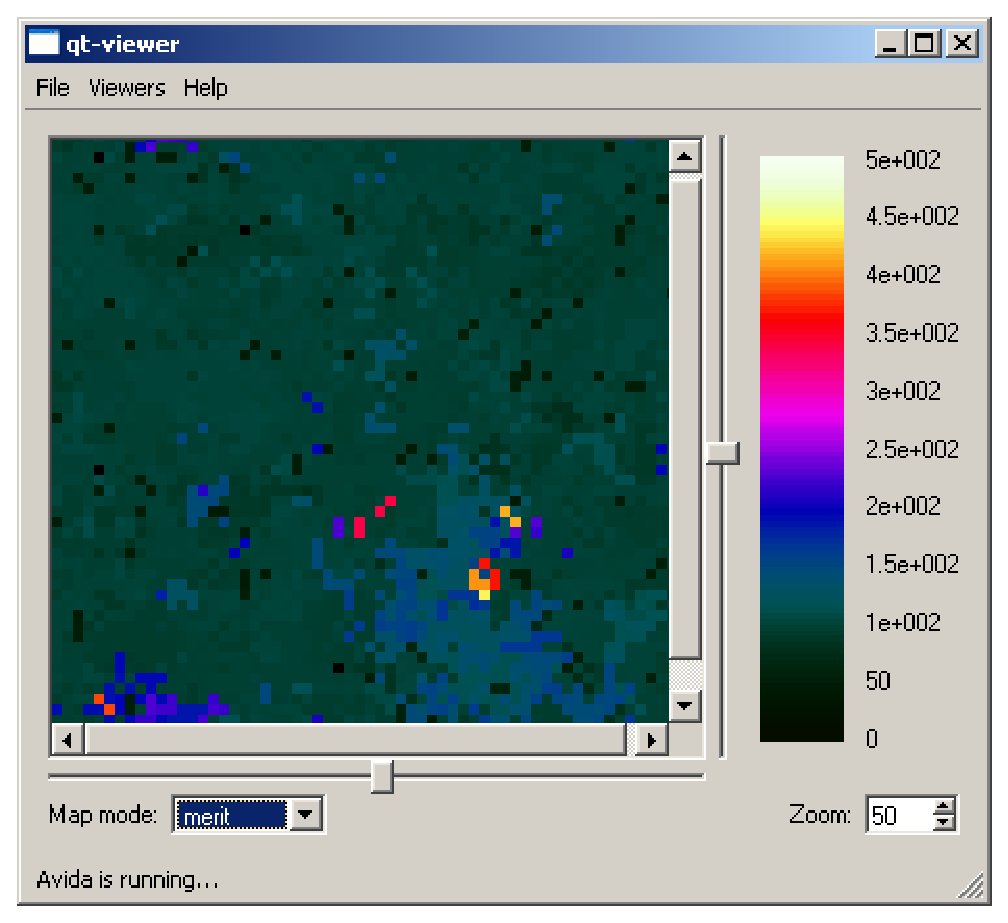
\includegraphics[scale=0.5]{images/AvidaGUI.eps}
  \caption{Avida 2.0b7 --- graphical viewer.}
  \label{img.Avida}
\end{center}
\end{figure}

\vspace{20pt}

\begin{tabular}{|p{150pt}|p{220pt}|}
\hline
\textbf{Agents}&segments of code in a simple language called strings  \\ \hline
Body&one cell in the grid of the environment \\ \hline
Moving&no \\ \hline
Behavior&execution of the code \\ \hline
Features&content of stack and registers \\ \hline
Life-span&not restricted \\ \hline
Genes&string is itself a genome \\ \hline
Phenotypic space&any finite string constructed of instruction of the language. \\ \hline
Learning&no \\ \hline 
\end{tabular}
 
\vspace{10pt}
\begin{tabular}{|p{150pt}|p{220pt}|} 
\hline \textbf{Mating}& \\ \hline
Number of parents&1 \\ \hline
Number of offsprings&1 \\ \hline
Genetic algorithm&Poisson-random mutation \\ \hline
Choice of partner&no \\ \hline
Conditions of mating&no \\ \hline
Investment in offspring&no \\ \hline 
\end{tabular} 

\vspace{10pt}
\begin{tabular}{|p{150pt}|p{220pt}|} 
\hline 
\textbf{Environment}& \\ \hline
Description&a grid of cells in the form of torus \\ \hline
Features&resources and tasks, completion of a task gives a bonus to the string \\ \hline
Inhabitants&strings \\ \hline 
\end{tabular} 

\vspace{10pt}
\begin{tabular} {|p{150pt}|p{220pt}|}\hline \textbf{UI settings}& \\ \hline
Mating&mutation rate \\ \hline
Life of individual&initial genomes of initial individuals \\ \hline
Environment&resources and tasks of the environment \\ \hline 
\end{tabular} 

\vspace{10pt}
\begin{tabular} {|p{150pt}|p{220pt}|}\hline \textbf{Statistics}&instruction viewer, string details, etc. \\ \hline
\end{tabular} 

\vspace{10pt}
\begin{tabular}{|p{150pt}|p{220pt}|} \hline \textbf{Implementation}& \\ \hline
Distribution of computation&no \\ \hline
Speed settings&console version versus GUI version  \\ \hline
Available sources&yes \\ \hline
Availability of binaries&free \\ \hline
Programming language&C++ \\ \hline
\end{tabular}

%*****Opening paragraph about every simulator: 
 %Name and version that I examined, 
 %url address
 %author
 %categorization into 3 systems

\subsection {Bitozoa}
Bitozoa is a simulator created by M. Borkowski, that uses for representation of agents neural network in combination with a set of parameters. It evolves two types of agents, herbivores and carnivores. It was created for purpose of amusement and education. Used version is Bitozoa 2 --- artificial life and artificial intelligence simulation, 2000. Web page of the project is \url{http://www.bpp.com.pl/bitozoa2/bitozoa2.html}.

\begin{figure}
\begin{center}
  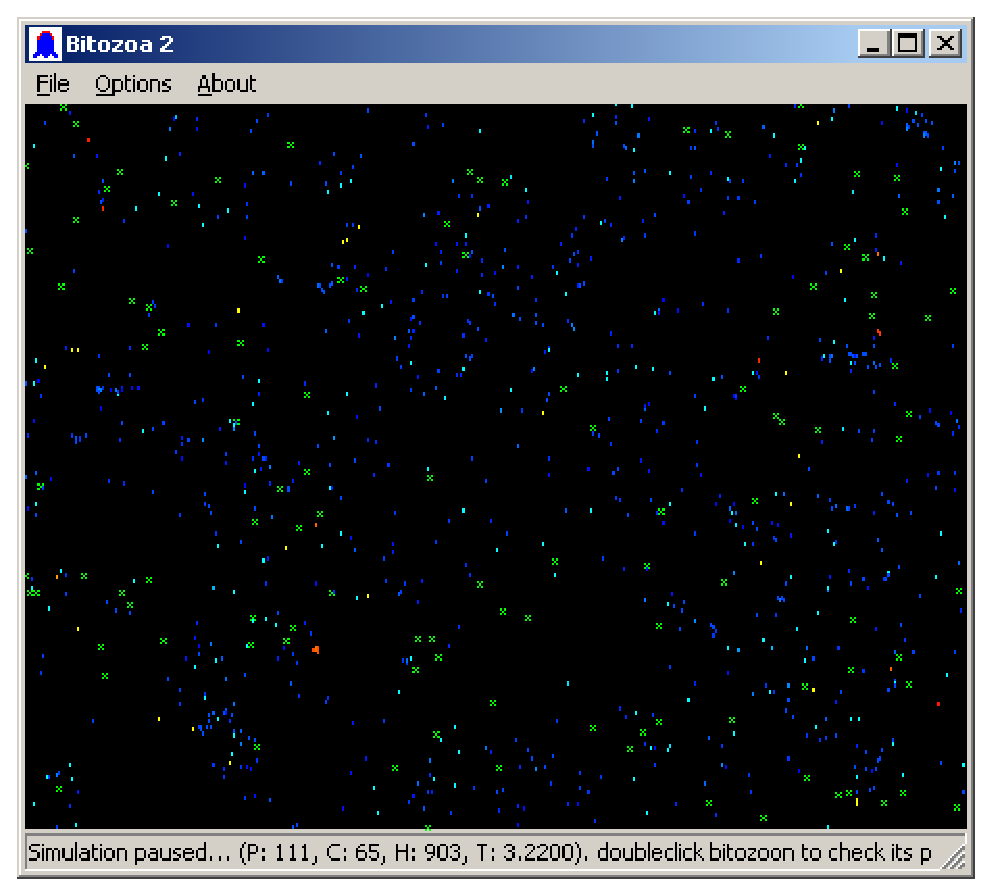
\includegraphics[scale=0.5]{images/Bitozoa.eps}
  \caption{Bitozoa 2.}
  \label{img.Bitozoa}
\end{center}
\end{figure}

\vspace{20pt}
\begin{tabular}{|p{150pt}|p{220pt}|}
\hline
\textbf{Agents}&Bitozoa --- herbivores (eat plants) and carnivores (eat herbivora)\\ \hline
Body&ball with 5 eyes, 2 flagella, various number of neurons, neural network with various topology. Eyes see all object in the world.\\ \hline
Moving&moves using flagella\\ \hline
Behavior&no\\ \hline
Features&energy level --- for moving and work of neurons, burned with speed according to age \\ \hline
Life-span&(?)\\ \hline
Genes&(?)\\ \hline
Phenotypic space&angle of flagella connection to body, number of neurons, topology of neural network, sensitivity of eyes\\ \hline
Learning&no\\ \hline
\end{tabular} 

\vspace{10pt}
\begin{tabular}{|p{150pt}|p{220pt}|}
\hline 	\textbf  {Mating}&\\ \hline
Number of parents&2 or 1\\ \hline
Number of offsprings&1--n (2 parents) or 1 (1 parent)\\ \hline
Genetic algorithm&random number of genes from both parents + mutation\\ \hline
Choice of partner&same species and high enough stamina\\ \hline
Conditions of mating&meeting of two bitozoa \\ \hline
Investment in offspring&both parents give the same fixed amount\\ \hline
\end{tabular} 

\vspace{10pt}
\begin{tabular}{|p{150pt}|p{220pt}|}
\hline 	\textbf  {Environment}&\\ \hline
Description&space in the form of a toroid\\ \hline
Features&number of spots, where food grows\\ \hline
Elements&food growing on special spots, herbivores and carnivores\\ \hline
\end{tabular}
 
\vspace{10pt}
\begin{tabular}{|p{150pt}|p{220pt}|}
\hline 	\textbf  {UI settings}&\\ \hline
Mating&breed distance, breed level of stamina, inherited stamina\\ \hline
Life of individual&asexual reproduction allowed, costs of an action, flagella angle and efficiency, view of bitozoa, adding or killing of a bitozoa, stamina from food, strength of carnivore, initial values of: eye sensitivity, number of neurons and stamina\\ \hline
Environment&number of bitozoa and food spots at the beginning, time increment, viscosity, random numbers generator seed\\ \hline
\end{tabular} 

\vspace{10pt}
\begin{tabular}{|p{150pt}|p{220pt}|}
\hline 	\textbf  {Statistics}&graph of population, energy flow and energy flow averaged, simulation description\\ \hline
\end{tabular} 

\vspace{10pt}
\begin{tabular}{|p{150pt}|p{220pt}|}\hline 	
\textbf  {Implementation}&\\ \hline
Distribution of computation&no\\ \hline
Speed settings&animation on-off\\ \hline
Available sources&partially\\ \hline
Availability of binaries&permission from author\\ \hline
Programming language&C++ Win32API\\ \hline
\end{tabular}

\subsection {Gene Pool}
Gene Pool was created by Jeffrey Ventrella, current version is 5. It is a parameter based simulator, dealing with evolution of swimming creatures in a virtual Darwinian aquarium. It is a game with intriguing graphical interface, san serve as an entertaining learning tool, but author demonstrated with it also several interesting results concerning influence of attractiveness of partners on  results of evolution.\cite{GenePool1} \cite{GenePool2}

\begin{figure}
\begin{center}
  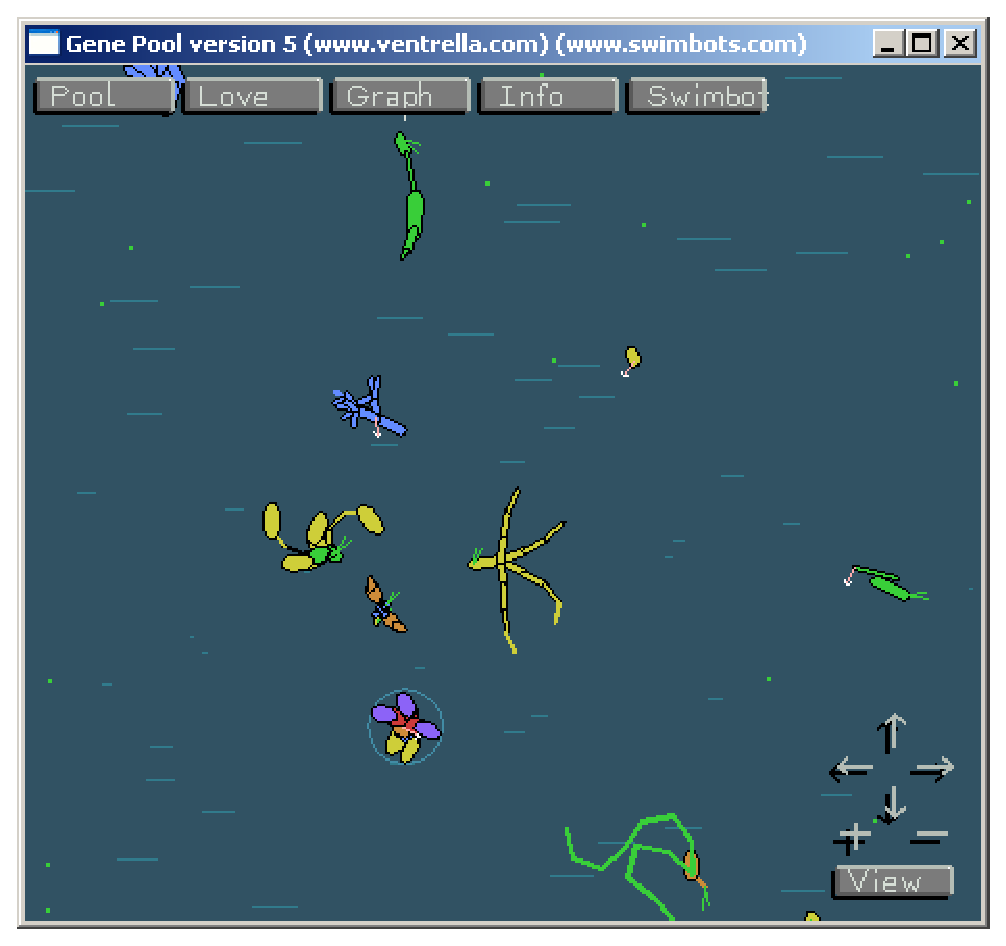
\includegraphics[scale=0.5]{images/GenePool.eps}
  \caption{Gene Pool 5.}
  \label{img.GenePool}
\end{center}
\end{figure}
  
\vspace{20pt}
\begin{tabular}{|p{150pt}|p{220pt}|}
\hline
\textbf{Agents}&swimbots\\ \hline
Body&mouth, genitals and 2--10 parts for moving\\ \hline
Moving&swimming using parts, algorithm common for all swimbots\\ \hline
Behavior&nothing\\ \hline
Features&energy\\ \hline
Life-span&not restricted\\ \hline
Genes&(?)\\ \hline
Phenotypic space&length, width, phases, amplitudes and attachment of every part\\ \hline
Learning&no\\ \hline
\end{tabular} 

\vspace{10pt}
\begin{tabular}{|p{150pt}|p{220pt}|} \hline \textbf{Mating}&\\ \hline
Number of parents&2\\ \hline
Number of offsprings&1\\ \hline
Genetic algorithm&crossover algorithm with mutation\\ \hline
Choice of partner&swimbot chooses at one snapshot in his view horizon one mate that most satisfies his attractiveness criterion\\ \hline
Conditions of mating&swimbots mate when at least one of them is pursuing the other and the distance between their genitals is less than the length of the genital vector\\ \hline
Investment in offspring&50\% of actual energy\\ \hline
\end{tabular} 

\vspace{10pt}
\begin{tabular}{|p{150pt}|p{220pt}|} \hline \textbf{Environment}&\\ \hline
Description&rectangular pool\\ \hline
Features&constant amount of energy in environment, cycle: food --- swimbots --- pool --- food\\ \hline
Elements&food bits, swimbots\\ \hline
\end{tabular} 

\vspace{10pt}
\begin{tabular}{|p{150pt}|p{220pt}|} \hline \textbf{UI settings}&\\ \hline
Mating&attraction criterion\\ \hline
Life of individual&location in environment, creation a swimbot, hunger threshold, energy for offspring\\ \hline
Environment&food growth --- birth delay, spread radius, energy from 1 piece\\ \hline
\end{tabular} 

\vspace{10pt}
\begin{tabular}{|p{150pt}|p{220pt}|} \hline \textbf{Statistics}&graph of number of swimbots vs. food, features of individual, the best one in attraction/mating/eating\\ \hline
\end{tabular} 

\vspace{10pt}
\begin{tabular}{|p{150pt}|p{220pt}|} \hline \textbf{Implementation}&\\ \hline
Distribution of computation&no\\ \hline
Speed settings&no\\ \hline
Available sources&no\\ \hline
Availability of binaries&yes\\ \hline
Programming language&(?)\\ \hline
&\\ \hline


\end{tabular}

\subsection {Mitozoos}
The author of project Mitozoos is Spanish software company Bestiario. Purpose of the simulator is educational, as author states "Mitozoos is an interactive artificial life model created with the objective that through experimentation and play participants will understand the relationship between genetic code and life." The web presentation of the project can be found at \url{http://bestiario.org/mitozoos/english/index.html}.

\begin{figure}
\begin{center}
  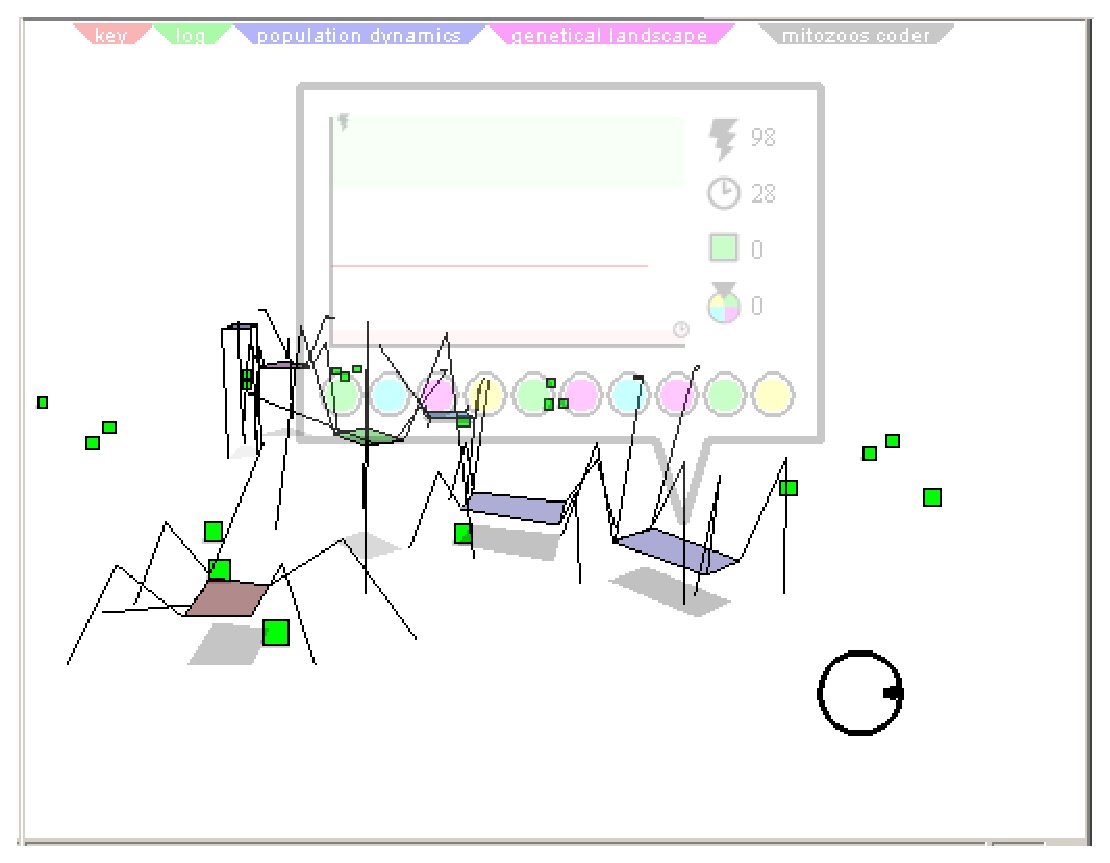
\includegraphics[scale=0.5]{images/Mitozoos.eps}
  \caption{Mitozoos.}
  \label{img.Mitozoos}
\end{center}
\end{figure}

\vspace{20pt}
\begin{tabular}{|p{150pt}|p{220pt}|}
\hline
\textbf{Agents}&mitozoos \\ \hline
Body&spider-like, with 2 eyes, body in shape of tetrahydron and four bent legs \\ \hline
Moving&walking using legs, algorithm common for all mitozoos \\ \hline
Behavior&strategy of eating, frequency and duration of resting periods \\ \hline
Features&energy \\ \hline
Life-span&not restricted \\ \hline
Genes&ten genes, each gene has four bases represented by colors \\ \hline
Phenotypic space&length of parts of legs, procreation threshold, eating strategy \\ \hline
Learning&no \\ \hline
\end{tabular} 

\vspace{10pt}
 \begin{tabular}{|p{150pt}|p{220pt}|} \hline \textbf{Mating}& \\ \hline
Number of parents&2 \\ \hline
Number of offsprings&1 \\ \hline
Genetic algorithm&crossover algorithm with mutation \\ \hline
Choice of partner&no \\ \hline
Conditions of mating&meeting of two mitozoos with energy higher than procreation threshold \\ \hline
Investment in offspring&a fixed amount of energy \\ \hline
\end{tabular} 

 \vspace{10pt} \begin{tabular}{|p{150pt}|p{220pt}|} \hline \textbf{Environment}& \\ \hline
Description&space in the form of a circle \\ \hline
Features&rate of food growth \\ \hline
Elements&mitozoos, food bits \\ \hline
\end{tabular} 

 \vspace{10pt}
 \begin{tabular}{|p{150pt}|p{220pt}|} \hline \textbf{UI settings}& \\ \hline
Mating&no \\ \hline
Life of individual&special application, which avails user to create a mitozoos by setting its genes and add it to running life. \\ \hline
Environment&initial number of mitozoos and food pieces, food growing rate, mutation rate \\ \hline
\end{tabular} 

 \vspace{10pt}
 \begin{tabular}{|p{150pt}|p{220pt}|} \hline \textbf{Statistics}&graph of number of swimbots vs. food, features of individual, genetic landscape, log of events, on reproduction join crossjoin of genotypes is shown \\ \hline
\end{tabular} 

 \vspace{10pt}
 \begin{tabular}{|p{150pt}|p{220pt}|} \hline \textbf{Implementation}& \\ \hline
Distribution of computation&no, but coders can run on different computers. \\ \hline
Speed settings&no \\ \hline
Available sources&no \\ \hline
Availability of binaries&yes \\ \hline
Programming language&Action Script, (?) \\ \hline
\end{tabular}

\subsection {Primordial Life}
For following evaluation Primordial Life 3.0 by Jason Spofford was tried. It can be downloaded at \url{http://www.io.com/~spofford/prim30.html}. Primordial life is a shareware parameter based artificial life screen saver written for purpose to capture the principles of evolution in an interesting and visual way.

\begin{figure}
\begin{center}
  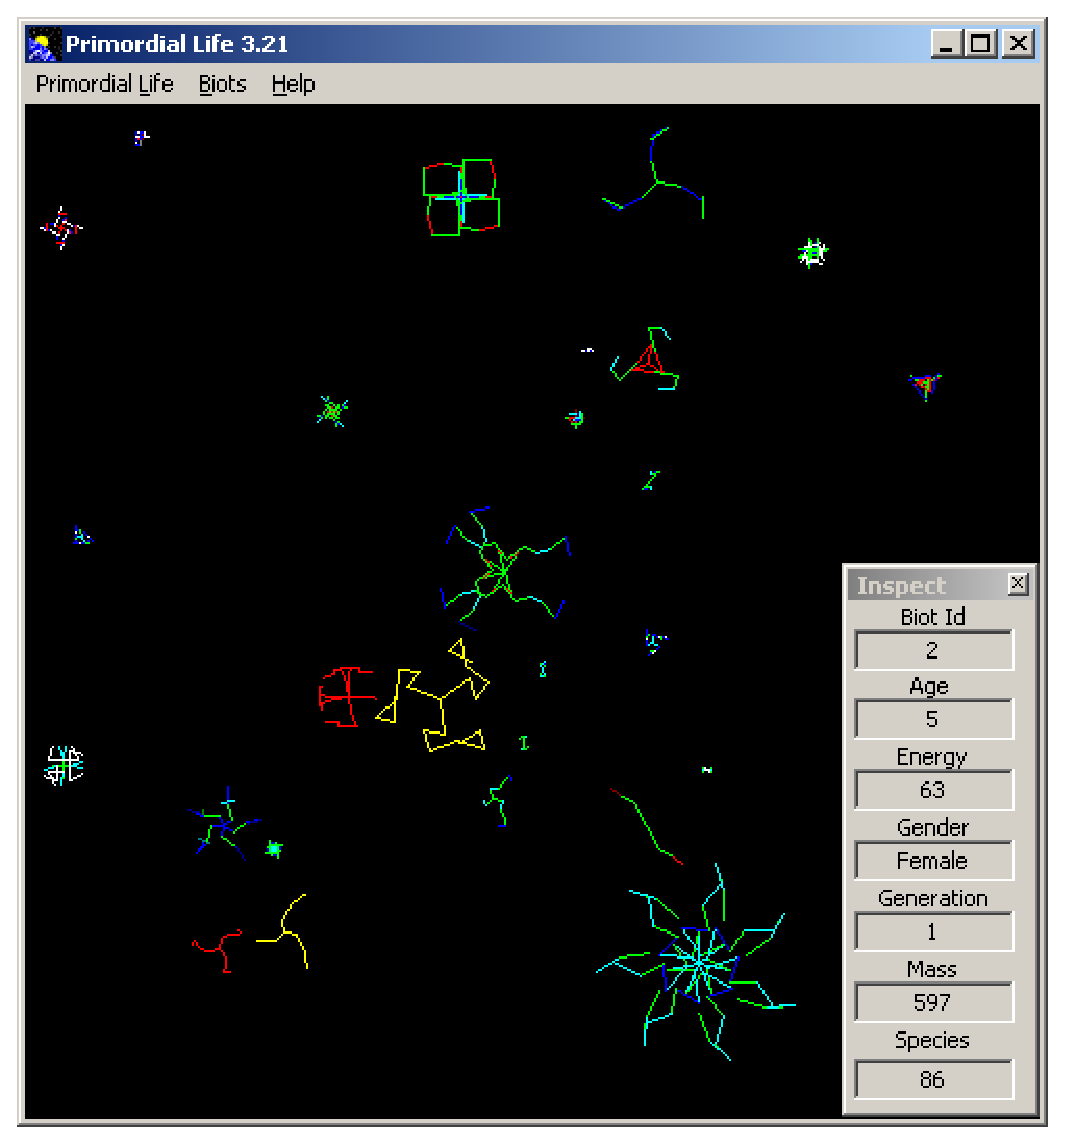
\includegraphics[scale=0.5]{images/PrimordialLife.eps}
  \caption{Primordial Life 3.21.}
  \label{img.PrimordialLife}
\end{center}
\end{figure}


 
\vspace{20pt}
 \begin{tabular}{|p{150pt}|p{220pt}|}
\hline
\textbf{Agents}&biots\\ \hline
Body&pattern of vectors of different colors, color of a part determines its special function.\\ \hline
Moving&moved by environment or by its motor (light blue parts)\\ \hline
Behavior&fighting with each other\\ \hline
Features&energy level\\ \hline
Life-span&restricted\\ \hline
Genes&64 numbers, describe lines color, orientation and length. Certain genes have special meaning detailing how many lines a biot has, its symmetry, whether it has mirrored or radial symmetry, how many children it should have and whether or not it should disperse its children after they are born. Complete description available.\\ \hline
Phenotypic space&number and symmetry of vectors, color, orientation and length of each vector, number and dispersion of offspring in a birth\\ \hline
Learning&learn from collision with other biots\\ \hline
\end{tabular} 

 \vspace{10pt}
 \begin{tabular}{|p{150pt}|p{220pt}|} \hline \textbf{Mating}&\\ \hline
Number of parents&2 or 1\\ \hline
Number of offsprings&1--n\\ \hline
Genetic algorithm&genetic crossover with mutation (2 parents), mutation (1 parent)\\ \hline
Choice of partner&no\\ \hline
Conditions of mating&collision of two biots, one of them with white parts\\ \hline
Investment in offspring&yes\\ \hline
\end{tabular} 

 \vspace{10pt}
 \begin{tabular}{|p{150pt}|p{220pt}|} \hline \textbf{Environment}&\\ \hline
Description&rectangular space\\ \hline
Features& mixing of biots continually up and providing of light, absorbable by green parts of biots and used up as energy\\ \hline
Elements&biots\\ \hline
\end{tabular} 

 \vspace{10pt}
 \begin{tabular}{|p{150pt}|p{220pt}|} \hline \textbf{UI settings}&\\ \hline
Mating&mutation rate, sexual/asexual/ both reproduction\\ \hline
Life of individual&life span, speed, regeneration rate and cost, attacking of child, battle of siblings, level of selfchange thanks to collision\\ \hline
Environment&solar intensity, friction, starting population, plague --- its duration and lethality\\ \hline
\end{tabular} 

 \vspace{10pt}
 \begin{tabular}{|p{150pt}|p{220pt}|} \hline \textbf{Statistics}&ecosystem status (population, death and birth rate numbers), global status of all connected ecosystems (no. of connected ecosystems, population)\\ \hline
\end{tabular} 

 \vspace{10pt}
 \begin{tabular}{|p{150pt}|p{220pt}|} \hline \textbf{Implementation}&\\ \hline
Distribution of computation&connection of ecosystems in a network over the Internet.\\ \hline
Speed settings&no\\ \hline
Available sources&no\\ \hline
Availability of binaries&register\\ \hline

%do porovnani:&"  A Primordial Life Server provides lists of available ecosystems you can connect with.   Ecosystems still connect peer to peer& the server just provides addresses of other ecosystems willing to let you connect with them. Advanced setting available !!"\\ \hline
\end{tabular}

\section{Features of Abeetles}
%Abeetles is a successor of Broucci(bez pameti)
The original idea of Abeetles is to create a successor of existing program Broucci (= Beetles) introduced by Tom\'{a}\v{s} Holan as an example of a different attitude to solution of complex problems. It is not an artificial life simulator, but it could be classified as a related system. It uses genetic programming to solve a specifical problem. The assignment of Broucci is that there is a world where beetles live. Beetles can move --- make a step, rotate left and rotate right. The step can head for an empty space or to eat a beetle and occupy its place. They can see what is around them --- in the front, on the left and on the right. Task is to find an algorithm that should a beetle use so as not to die of hunger and not be eaten up by another beetle. Solution described by the author is a console program where beetles are visualized as arrows turned in the direction of their sight. Beetles take turns regularly and always when the number of beetles goes down under certain level, new beetles are created from the most successful ones using genetic crossover algorithm. Parents do not meet.\cite{Broucci}

\begin{figure}
\begin{center}
  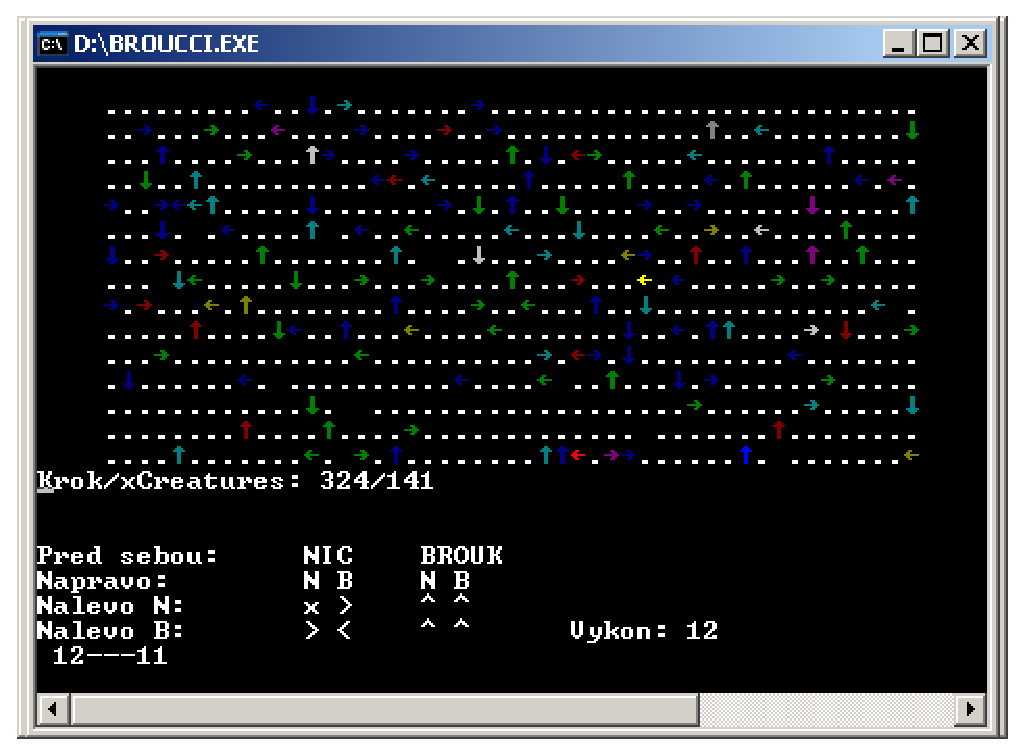
\includegraphics[scale=0.5]{images/Broucci.eps}
  \caption{Broucci.}
  \label{img.Broucci}
\end{center}
\end{figure}

Abeetles takes over following ideas of Broucci: beetles can move by sequence of steps and rotations. According to what they see is in the front, on the left and on the right do they decide which action to take. 
 
%Jak propojit navaznost na broucky s vmezerenim se mezi existujici programy? Posloupnost je jasna: 1. urcit, v cem chci na predchozi program navazat. 2. Rozvinout ho tak, aby zajimave vplynul mezi existujici simulatory.

"Brother programs" were compared according to 27 different cathegories. Abeetles does not strive to be contributing in all these categories. Instead of it, six were chosen as the key ones: moving, learning, choice of partner, distribution of computation, obstacles in environment and aging. The following table compares Abeetles with other solutions only using these categories.

\vspace{10pt} 
\begin{tabular}{lcccccc}
 & Avida & PLife&  Bitozoa& Mit.& GPool & Abeetles\\ \hline
Moving: strategy&x&x&G&S&S&G\\
Learning&x&O&x&x&x&G/O\\
Choice of partner&x&x&x&x&O&G\\
Distribution&x&Y&x&x&x&x\\
Obstacles&x&x&x&x&x&O\\
Aging&x&x&x&x&x&O\\
\end{tabular}
\vspace{10pt}

O --- optional (user can influence it), S --- static (fixed), G --- genetically evolved, x --- not present, Y --- yes

\vspace{10pt}

Moving strategy is a function of an organism, where input is the view and state of the organism and output is a decision what to do. Bitozoa evolve such a function genetically, but bases it on neural networks. Mitozoos uses fixed strategy that is influenced by several parameters. These parameters, e.g. maximal distance of a food bit in the view so as to head for it, are subject to evolution. Gene Pool has also fixed strategy. Abeetles overtake the idea of evolution of strategy of moving from its predecessor Broucci and intends to explore it.

Learning is a feature that is usually connected with neural networks. Parameter based simulators generally do not use it. But influence of simple learning on evolution of moving might be interesting, therefore it is placed among objectives of Abeetles. The term learning is very general, Abeetles inspired its view of learning with memetic theory. 

The term meme was first coined by Richard Dawkins in 1976. Dawkins defined the meme as "a unit of cultural transmission or a unit of imitation"\cite{SelfishGene}. Memes have as an important characteristic their propagation through imitation, a concept introduced by the French sociologist Gabriel Tarde. Imitation involves copying the observed behavior of another individual. Researchers have observed memetic copying in just a few species on Earth, including hominids, dolphins and birds (which learn how to sing by imitating their parents). The technique of dissemination of memes in population can be formalized and it is described e.g. in lectures of Vlado Kvasnicka from CHTF STU at \url{ftp://math.chtf.stuba.sk/pub/vlado/Evol_alg_MFF/prednaska1_transp.pdf}.

Abeetles uses imitation of behavior in the way that agents copy some patterns of behavior from other more successful beetles. It would be interesting to explore, to which extent is mutual learning convenient. Abeetles adds probability of learning from another beetle to features of agents and evolves it.

Choice of partner for mating is the next idea Abeetles concerns with. In Primordial Life, Bitozoa and Mitozoos choice of partner is restricted to demand on sufficient level of energy of both parents. Gene Pool is on the other hand interested in influence of criterion of choice of partner on results of evolution. \cite{GenePool2} In contrast to it, Abeetles chooses fixed criteria and evolves their values.   

Simulator Primordial life offers possibility to connect simulators and in order to it connect environments together. The plan of Abeetles originally included computation distributed to more computers, but finally it is only a single computer application. Reasons are described later. 

Obstacles are incorporated in none of the five simulators. But obstacles and consequently the shape of the environment can be very interesting for Abeetles, which evolves strategy of motion.  

Aging is generally meant as dependence of performance of an agent on age. None of the five simulators implements it. Abeetles makes it possible for a user to set amount of energy obtained from food according to age of a beetle.

%Nemela bych jeste udelat presnou tabulku jako je u brother programs?

%%%%%%%%%%%%%%%%%%%%%%%%%%%%%%%%%%%%%%%%%%%%%%%%%%%%%%%%%%%%%%%%%%%%%%%%%%%%%
\chapter {Arificial Life in Abeetles}

This chapter describes the model of life in simulator Abeetles. It starts with basic ideas and continues to details and diagrams of the model.  

\section {Basic Ideas of the Model}

% Class diagram s entitami, jejich vztahy a integritnimi omezenimi.
\begin{figure}
\begin{center}
  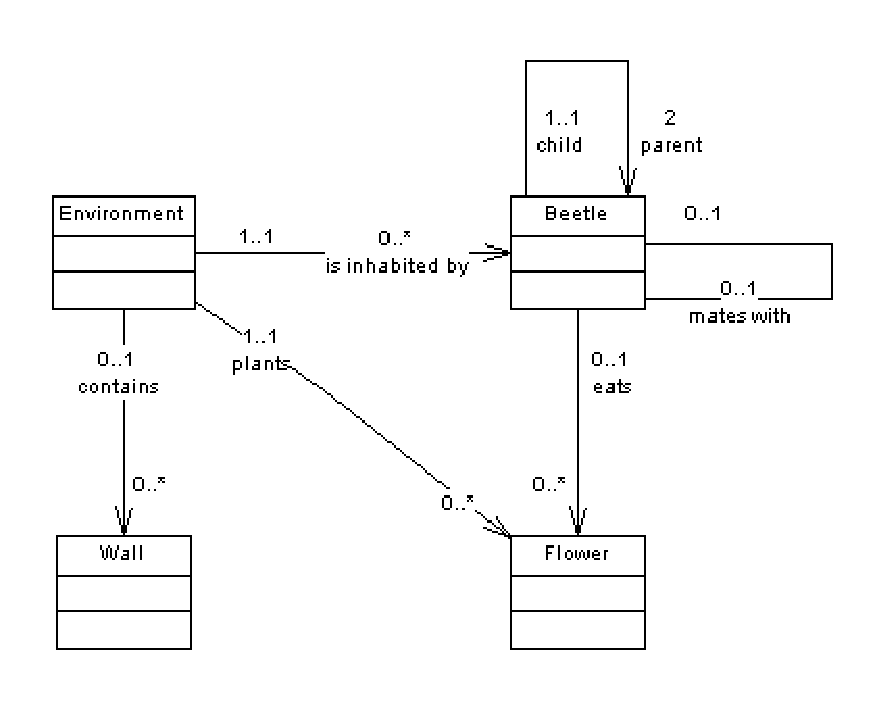
\includegraphics [scale=0.8]{images/AnalysisDataModel.eps} 
  \caption{Conceptual data model of Abeetles.}
  \label{obr.AnalysisDataModel}
\end{center}
\end{figure}

%Abeetles - simulator with agents and environment
Artificial life in simulator Abeetles is an environment inhabited by agents. Agents are the elements of environment that are subject to evolution and environment is all the space occupied by agents as well as not evolved objects. The conceptual model of key entities in Abeetles is shown in Figure \ref{obr.AnalysisDataModel}.

%Beetles - agents with static part and genome. Flowers. Walls
Agents in Abeetles are called beetles and generally they all are instances of the same model, as they share the same static part as well as constrains on the variable part of their behavior. The variable part makes up the genome and it is altered by evolution. It can be also influenced by learning. Relationships among beetles are created by mating and bearing of children. 

The environment is a grid in the form of a toroid. In the grid three types of objects are placed. Beetles are the only inhabitants of the environment that are able to move. Flowers grow in cells of the environment and serve as food for beetles. Neither beetles nor flowers can occur in cells of the grid where are walls. Walls are static obstacles that serve for forming of the shape of the environment.

\section{Brief Model of Abeetles}
%Beetle and its attributes, environment and its attributes
The basic model of life in Abeetles is described. Now decomposition proceeds and data structures are designed.
The key data structures of Abeetles are beetles and their environment.
A beetle has following evolvable features:
\begin {itemize}
\item Brain --- decision function that finds to every situation one action. The situation is a combination of what the beetle sees and of his inner states. States of a beetle are whether he is hungry or not. A beetle sees what is on the left,in the front and on the right, overall three cells of the grid of the environment.
\item Expectations on parter --- A beetle checks before mating whether the partner  fulfills its expectations on amount of energy, investment in children, learning ability and age.
\item Hungry threshold --- The threshold defines whether the beetle is or is not hungry.  
\item Investment in children --- A beetle invests this amount of energy into its new born offspring.
\item Learning Ability --- A beetle expects certain level of learning ability from its partner.
\end {itemize}

Evolvable features are concatenated into a chromosome. Process of mating and creation of genome of a child has three steps:

\begin{itemize}
  \item Selection --- beetles must meet and consider each other attractive using their feature expectation on partner. 
  \item Crossover --- There are several possible algorithms:
    \begin{itemize}
      \item One-point crossover: Standard algorithm chosen for Abeetles.
      \item Two-point crossover: This algorithm seems to be also useful for the case of Abeetles. It would be interesting to implement it, too, and compare results with the one-point algorithm. 
      \item "Cut and splice": This technique is not suitable for the case of Abeetles, because created children have different length of chromosomes.
      \item Uniform Crossover and Half Uniform Crossover: These aproaches may also be useful, but the standard one-point algorithm was preffered.
      \item Crossover for Ordered Chromosomes: This aproaches may also be interesting, but the standard one-point algorithm was preffered.
    \end {itemize}
  \item Mutation --- Genome of a new-born beetle is mutated.
\end {itemize}

%For implementation of crossover step the possible crossover points must be carefully chosen. The target is to find points, that availe separation of the genome into two noninteracting groups. Otherwise the crossover is not important for evolution and may be omitted.Points can be placed between any pair of adjacent variables. Two created parts will be independent


Non evolvable features of beetles are current direction in environment, e.a. east, north, west or south and amount of energy.

The Environment contains beetles, flowers, walls and empty cells. Flowers are objects in environment that serve as food for beetles. Similar source of energy for agents use Bitozoa, Gene Pool and Mitozoos. Gene Pool keeps a fixed amount of energy in the environment, the less agents the more food and vice versa. This attitude prevents users from exploring, how would agents develop with higher of lower supplies of food. In contrast to Gene Pool, in Abeetles can amount of food vary from zero to full grid of flowers. Due to demand on local interactions for purposes of possible parallelization, growth of flowers is an individual matter of every cell influenced only by general parameter. Each cell has an optional probability of growth of flowers. If it happens, the flower springs up in one update and occupies the cell until it is eaten or dies. Flower can die in any turn with fixed probability.  

Environment updates in turns. One update goes gradually, cell by cell. If a cell is empty, flower springs up with certain probability. When there is already a flower, it can with certain probability die. If the cell is occupied by a beetle, the beetle takes a snapshot of three neighboring cells and according to it and his hunger he decides what to do and carries it out. 

%Alternatives

\section{Detailed Design of Life of Abeetles}
%1st - Data model of Alife in Abeetles - UML Class diagram of attributes and methods of Environment, Grid and Beetles

Detailed design of life of Abeetles compounds three classes. CEnvironment, CGrid and CBeetle. UML Class diagram of all three classes and their relationships is in \ref{img.ClassDiagrAbeetlesAlife}. 

Class CGrid represents the grid of the environment. It stores its size and contents. The most important operations are GetFlowerGrowingProbability and GetCellContent, which returns what is placed in certain cell and in case it is a beetle, it returns reference to it. This class is designed to encapsulate prospective paralelization.

%Beetle's action
Class CBeetle represents a beetle with all respective features. Beetles make one action in every turn. It can be a step, a rotation or a mating. An attempt to mate happens every time, when a beetle sees another beetle in front of him. If the attempt is not successful, the beetle chooses another action according to his Brain. In the Brain only rotations and steps are included.

The possibility to place mating among other actions in the brain was tried for Abeetles, but it made it impossible for randomly created beetles to evolve, because only a small number of them received randomly the decision to mate in the suitable situation. And the number was not enought to keep the density of population in next generation above the border of extinction.

%Mating
The most interesting process connected with class CBeetle in mating of two beetles. First, demands of both beetles are checked by function IsExpOnPartnerSatisfied(). When beetles find themselves mutualy attractive,  operation CreateChild() is called. This method first applies Crossover1Point() containing a genetic crossover algorithm and generates two genomes. One of them is randomly chosen for the new-born descendant. The descendant then undergoes random changes in operation Mutation(). The new beetle is then placed in one of four cells that are neighboring for both parents. Afterwards it starts to live its own life.

%Run of life
Another important process in the environment is the run of life in the environment. Instance of class CEnvironment is called $env$. Its attribute Grid   contains the actual situation in the environment. Using the following code one update of the environment is performed.

\begin{verbatim}

for(I=0;I<Grid.G_Width;I++)
    for(J=0;J<Grid.G_Height;J++)
    {
      //if cell was not updated yet, update it.
      if ((Grid.IsCellUpdated(I,J))==false)
      {
        if (Grid.GetCellContent(I,J)==BEETLE) MakeBeetleAction(I,J);
        else if (Grid.GetCellContent(I,J)==NOTHING) MakeFlowerGrow(I,J);
        else if (Grid.GetCellContent(I,J)==FLOWER) MakeFlowerDie(I,J);
        //Mark the cell as updated one
        Grid.SetCellUpdated(I,J); 
      }
    }
		
\end{verbatim}		

The border between two updates is method NextTime() placed in class CEnvironment. Among others, it counts statistics of the previous turn.

\begin{figure}
\begin{center}
  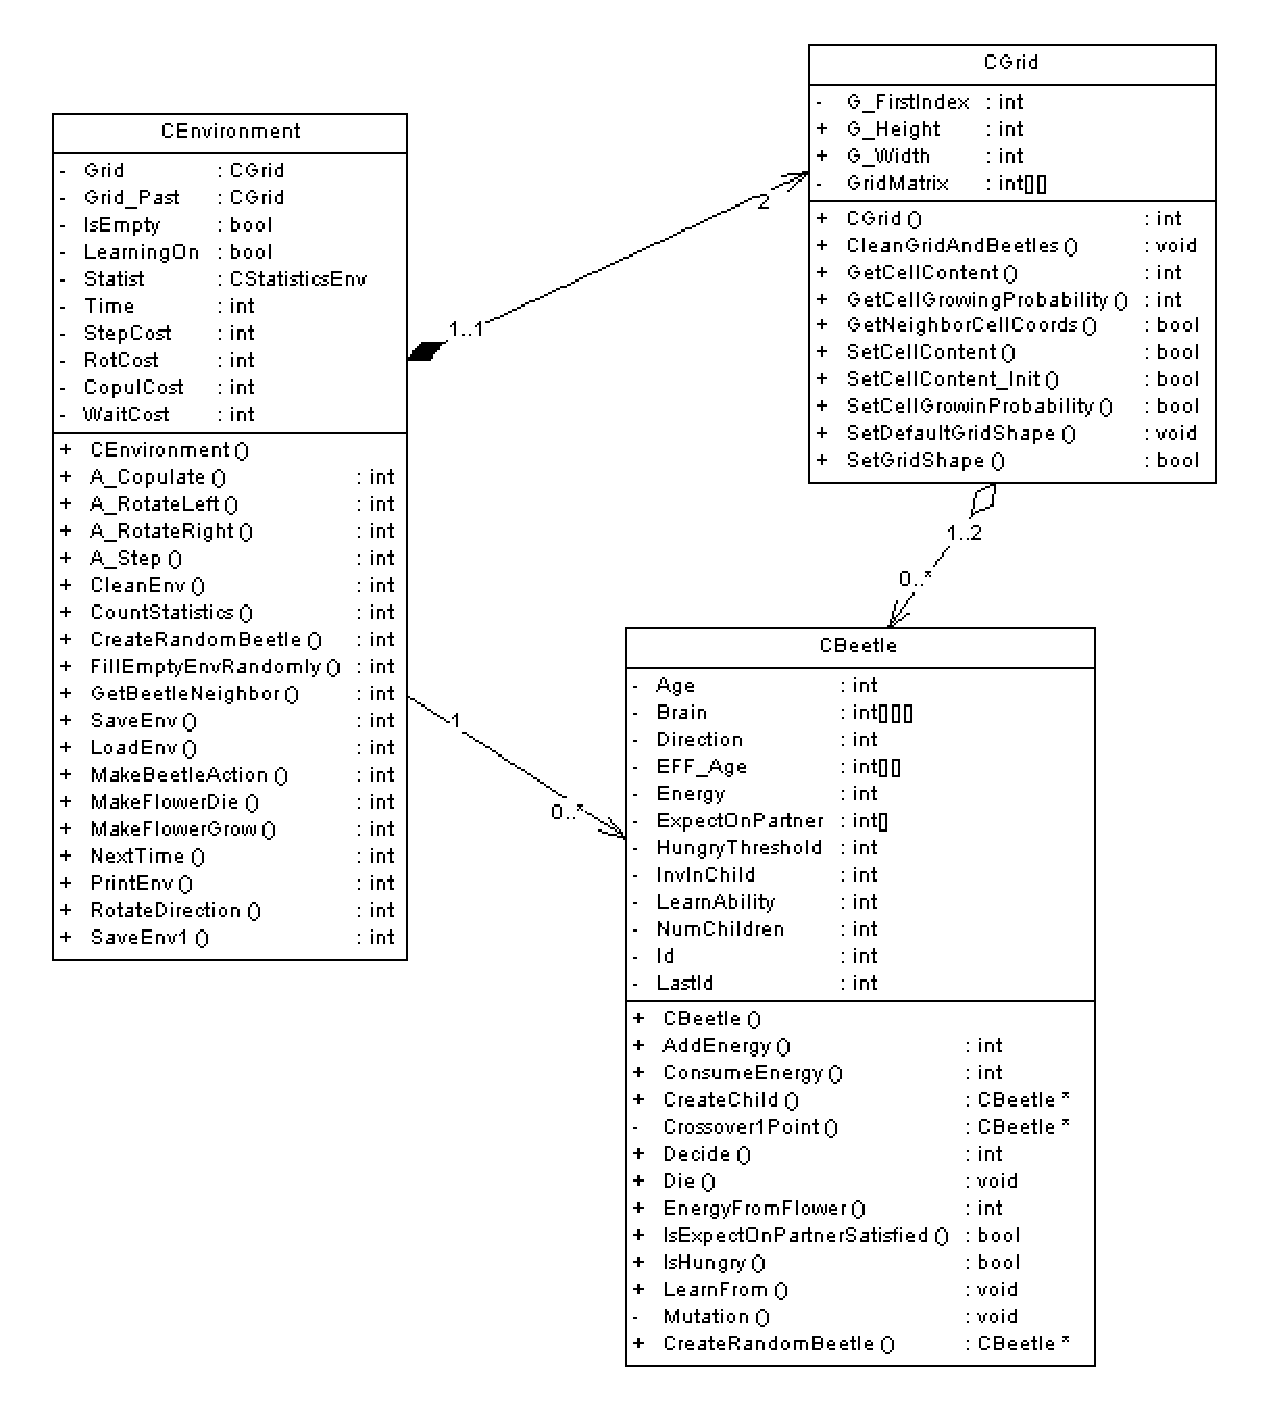
\includegraphics [scale=0.6]{images/ClassDiagrAbeetlesAlife.eps}
  \caption{Class diagram of Alife in Abeetles.}
  \label{img.ClassDiagrAbeetlesAlife}
\end{center}
\end{figure}


%%%%%%%%%%%%%%%%%%%%%%%%%%%%%%%%%%%%%%%%%%%%%%%%%%%%%%%%%%%%%%%%%%%%%%%%%%%%%
\chapter{Creation of Abeetles: Analysis}%Ten nazev se mi nelibi, co s nim? Jen "Analysis"? nebo "Design"?


\section{Functionality of Abeetles}

The simulator runs the model of life described above. Scenarios of usage can be encapsulated in three particular cases of usage: running of an experiment, view of an experiment, and learning of life in the simulator and usage of the application.
%A co soupnout napad tehle tri scenarii uz do Chapter 3?

\subsection {Running of an Experiment}
UML sequence diagram is shown in figure \ref{obr.ScenarioRunExperiment}.In this case, the expectations on the system are:
\begin{itemize}
\item Speed: Experiment run with the simulator should execute thousands of turns so as to get interesting results of evolution. Also for statistical purposes high number of various inputs must be used when experimenting on random data. Therefore Abeetles should offer very fast execution. 
\item Input: The start of experiments cannot be done manually one by one. Data entry should be read from a script. 
\item Output data: It should be possible to save results of experiments in an interchangeable format and make their collection automatically during execution.
\item Run of the simulator: The simulator should just obtain a script at the start and then run without need for any other input from the user. 

\end{itemize}

\begin{figure}
\begin{center}
  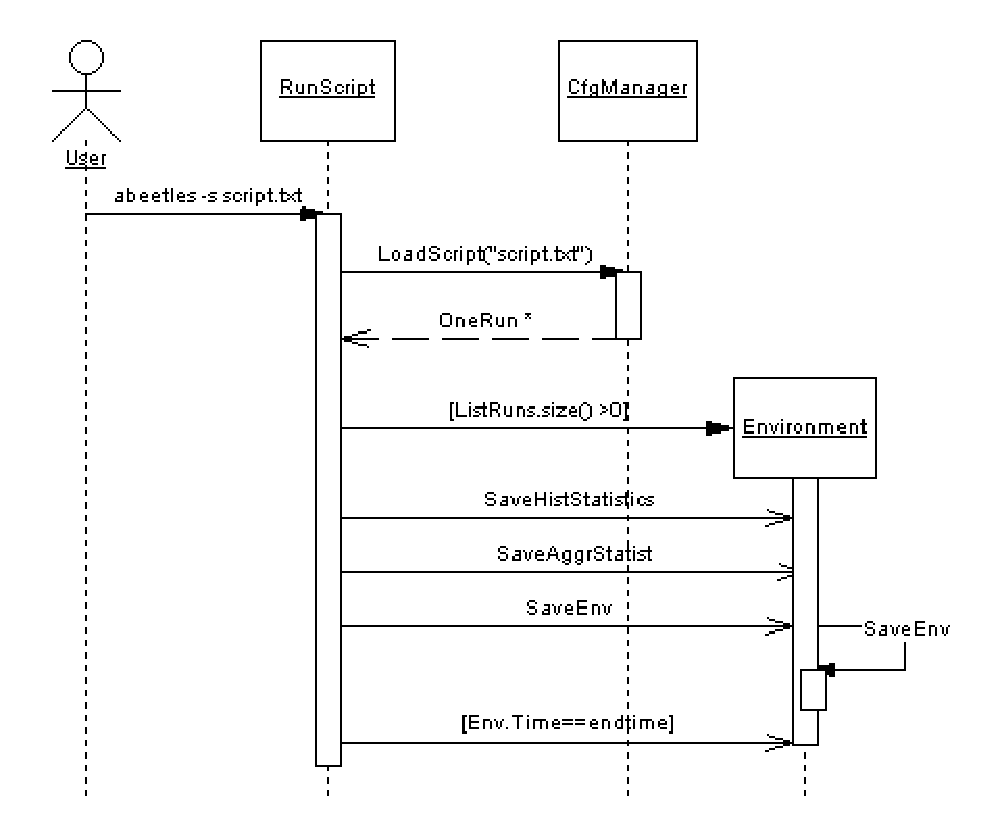
\includegraphics [scale=0.6]{images/ScenarioRunExperiment.eps} 
  \caption{UML Sequence diagram --- run of a script.}
  \label{obr.ScenarioRunExperiment}
\end{center}
\end{figure}
%Scenarion of running of an experiment - sequence diagram.

\subsection{View of an Experiment}
UML sequence diagram is displayed in figure \ref{obr.ScenarioRunExperiment}. Expectations:
\begin{itemize}
\item User interface: Interface should offer possibility to look at the environment with all its objects so as to see any particular situation in the environment that cannot be logged in statistics, e.g. differences between beetles in separate parts of the environment. This could be realized by ability to visualize different aspects of the environment on demand and by ability to zoom various parts of the environment. Also details of individual beetles should be accessible in a concise form. All suitable features should be possible to reset so as to observe step by step development under different conditions. 
\item Run of simulator: Simulator should be capable of running step by step, of running optional number of turns or of running until being stopped.
\end{itemize}

\begin{figure}
\begin{center}
  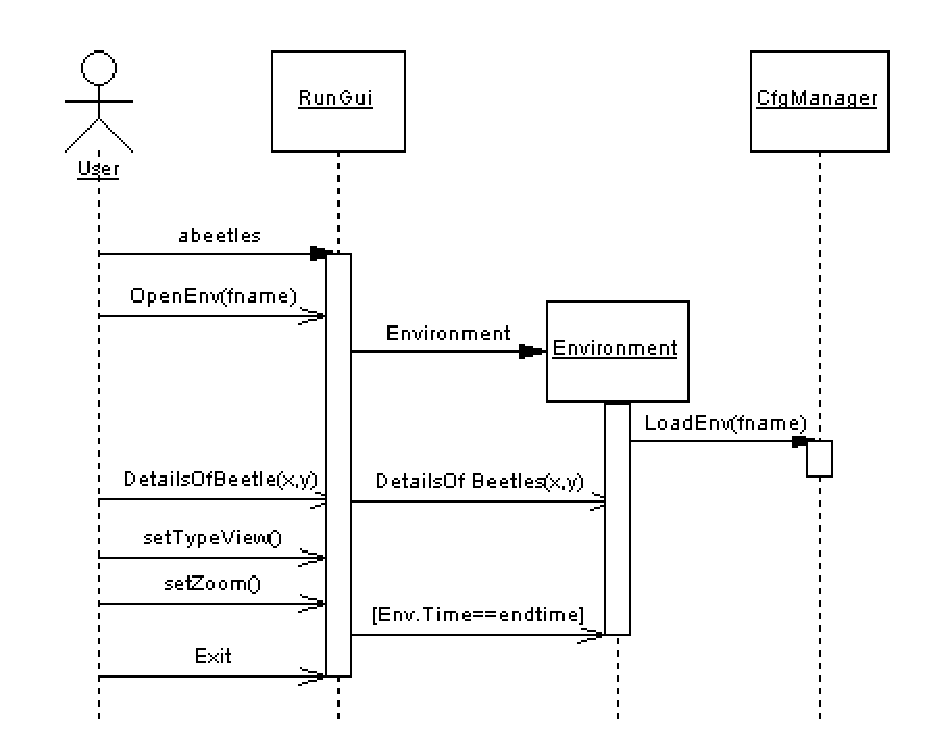
\includegraphics [scale=0.6]{images/ScenarioViewSituation.eps} 
  \caption{UML Sequence diagram --- view of a situation.}
  \label{obr.ScenarioViewSituation}
\end{center}
\end{figure}
%Scenario of view of an experiment

\subsection{Learning about Abeetles}
%aspect of understanding of the model and work of Abeetles.
\begin{itemize}
\item Speed: A slow run of the simulator helps to see what is happening and understand relationships between events.
\item User Interface: The interface should show all the environment with clearly differentiated objects. Legend, explaining what is what, should be easily reachable. A zoom can make possible to see the situation in details as well as to overlook the whole environment.
\item Input: Possibility to start default interface with random beetles easily is necessary at the beginning of work with the simulator. As well as the possibility to save the environment and load it so as to continue later.
\item Output: Actual statistics can be reached in any turn.  
\end{itemize}


%%%%%%%%%%%%%%%%%%%%%%%%%%%%%%%%%%%%%%%%%%%%%%%%%%%%%%%%%%%%%%%%%%%%%%%%%%%%%
\chapter{Creation of Abeetles: Design with Discussion of Alternatives}
%******************Návrh řešení s diskusí alternativ******************
\section{Architecture}


%Hardware architecture
  %Single computer 
  %Multiple computers
    %server+clients
    %peer to peer
\subsection {Hardware Architecture}

Abeetles is designed as an application that runs on a single computer, because it is tailored for only one user and for small amount of data. It does not need any special or demanding support. Only the demand on speed could be a reason for a more complicated solution. The simulator should be as fast as possible when running an experiment, but simultaneously it should be possible to go slowly and display a particular situation step by step. Speed can be from the point of view of hardware improved by parallelization of computation. This possibility was not realized, but might be interesting for future improvement of Abeetles. 

\subsection {Software Architecture}
%Software architecture
  %modules of application
    %1 module
    %2 applications
    %1 module + 1 computational library
  %language and GUI libraries
    % c++ 
      % + qt lib
      % + win32api
      % + mfc    
    % bytecode languages
      % Java
      % C#
\subsubsection {Modules of Abeetles}
Important facts from analysis that influence choice of layout of modules are usage as a tool for experiments, which expects fast run without visualisation, and usage as a viewer and a learning tool, which expects slow run with elaborate graphical interface. Separation of these two attitudes therefore comes into consideration.

Abeetles could be designed as a tool containing two separate applications that can only share some representation of data. First application is a graphical viewer and second one is a program that is run from a command line or a console application. This attitude is used by simulator Avida. Avida contains even three kinds of applications: graphical viewer, console application and primitive run with only listing of updates in a console.

Abeetles was first considered to be designed in this way. The console application could be written really primitively without any GUI concerned libraries and therefore could run very fast. Gui needs a supporting graphical library. For Abeetles the program language C++ together with graphical library Qt by Trolltech was used, as described in following section. This library, as well as Win32API or MFC, contains useful tools for work with files and parsing of text, which are necessary in both versions. To develop these operations for console version separately using non library constructs would be more difficult and time consuming, but without any real contribution. Therefore parallel development of two applications was abandoned. 

Division of application into modules could also follow separation of computation of artificial life from all wrapping functionality. The computation could be called as a dynamical library. For reuse of the core of Abeetles with different interface it would be convenient and it would also be suitable for cooperation of more developers. Abeetles are planned to be prepared for transfer to other operation systems, unix based or MacOS. And dynamical libraries are only usable at one system.

To sum up, Abeetles is an application that contains only one module that serves for both purposes --- running of experiments as well as overlooking individual situations in the environment and running step by step. Disadvantage is lower reusability, but it simplified development and thanks to chosen library conforms to future compilation on other operation systems.

%language and GUI libraries
    % c++ 
      % + qt lib
      % + win32api
      % + mfc    
    % bytecode languages
      % Java
      % C#
\subsubsection{Choice of Platform and Programming Language}

Platform for Abeetles is MS Windows XP. Thanks to usage of Qt library it should be possible to compile Abeetles for other OS in future.

Speed was the leading criterion when the question of programming language was considered. The model of Abeetles invokes realization by a class based languages, the abstraction is then intuitive. Abeetles needs graphical interface and for the chosen language a library for creation of GUI should be accessible. Three languages were taken into account: Java, C\# and C++. Both Java and C\# are, thanks to interpretation of bytecode at runtime, slow in comparison with C++. But a Java application can be run at different OS and it is a language with many convenient features. e.g. garbage collector. The criterion of speed was considered crucial for Abeetles and therefore C++ was chosen.

Graphical user interface in Abeetles is created using library Qt by Trolltech. Is offers encapsulating class based abstraction of interface and can be used for MS Windows, MacOS Unix and many Unix based platforms. Details are published at Trolltech's webpage \url{http://trolltech.com/products/qt}. Abeetles uses the open source version of Qt, which demands compilation using MinGW, \url{http://mingw.org/}.

Other possibilities were Win32API and MFC. The first is not class based and is difficult to use. MFC is a class based library, it is distributed freely with MS  Visual Studio, but the level of abstraction is lower than in Qt and Microsoft now prefers usage of .NET to usage of this library.

Graph algorithms used in Abeetles are realized using Boost C++ library, \url{http://www.boost.org/}. This library is designed for usage in C++ programs and compilation by MinGW is supported. 


\section {Components}
%Layout of functionality into classes CEnvironment, CRunScript, MainWindow, CGrid, CStatistics and CBeetle + alternatives.

\begin{figure}
\begin{center}
  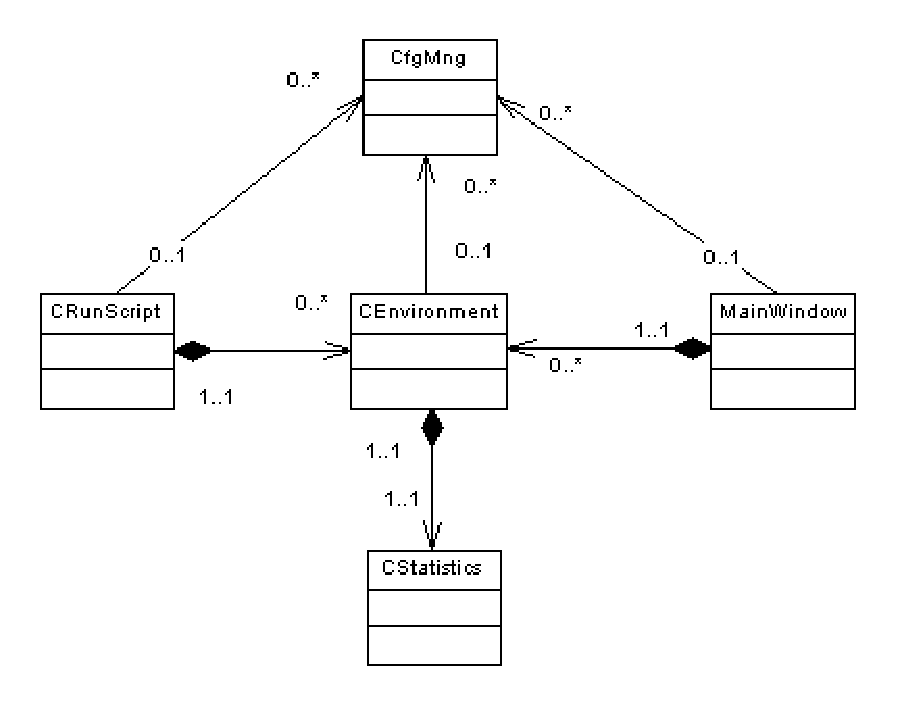
\includegraphics [scale=0.8]{images/ComponentModel.eps} %
  \caption{Diagram of main classes of Abeetles.}
  \label{img.ComponentModel}
\end{center}
\end{figure}

Functionality of Abeetles is divided into following components: Environment, Run of Script, Run of Gui, Statistics and Configuration Manager. Configuration Manager encapsulates functions for saving and loading of environments and scripts. Each of these components is  represented by its key class, see figure \ref {img.ComponentModel}.

\section {User Interface}
\subsection {Graphical User Interface}
The idea of graphical user interface of Abeetles was inspired by interface of Broucci, see figure \ref{img.Broucci} on page \pageref{img.Broucci}, regarding visualization of beetles. In Abeetles agents are also represented by arrows showing their direction. %figure

Layout of the window of GUI of Abeetles resembles the qt-view of Avida,  see Figure \ref{img.Avida} on page \pageref{img.Avida} . The reason is the similarity of grid base of environments and intention to serve as a scientific tool.

 
\subsection {Statistics}

Every artificial life simulator, that endeavors after more than being just a game, includes some kind of statistics. 
Systems compared with Abeetles display information either graphically or output them to a file (indicated in brackets):

\begin{itemize}
\item Avida: instruction viewer, details of individual strings 
\item Bitozoa: graph of populations, energy flow and energy flow averaged, information about environment (to file), details about an agent
 \item Gene Pool: graph of relationship between number of swimbots and amount of food, features of individual agents, to seek the best agent in chosen criteria
\item Mitozoos: genetic landscape, log of events, on reproduction the crossjoin of genotypes is shown graphically, details about an agent
\item Primordial life: information about the environment (population, time death and birth rate numbers), global status of all connected ecosystems, information about an agent
\end {itemize}

%Possible to add pictures of statistics from other programs.

These simulators prefer to show statistics graphically or textually in the program. But for further processing, output to files in a standard format might be more useful. Abeetles writes statistics into files, only several actual numbers shows in the graphical interface. Abeetles, as well as all described simulators, shows details of an individual, besides all other statistics. The first type of statistics offered by Abeetles is actual information about environment --- time, number of agents, number of flowers and average values of features of beetles. The second type are graphs of development in time that are very useful for observation of what is going on in the simulator within time. They are also offered by Bitozoa and Gene Pool. In contrast to them, Abeetles does not show graphs directly, but saves values into a file in comma separated value format. Graphs can be then drawn by a special program, e.g. MS Excel. In this format changes of number of beetles, number of flowers and number of births within time are stored. It is also used for graphs displaying frequency of distribution of values of age, learning abilities, investment in children and energy. Data in output files are precise without any modifications and can be  further proccessed by additional software.



  
\subsection {Script}

Script for Abeetles is intended to be easy to understand. It uses format
"command = value" or only "command" and facilitates gradual start of any number of runs of the simulator. For each of them all necessary parameters can be defined.

The alternative of usage of command line parameters instead of an Abeetles specific script was considered. One command could start one run of Abeetles and a set of runs could be created in a command line script. But the first alternative was chosen, because it makes it possible to write the script without knowledge of system commands.


%%%%%%%%%%%%%%%%%%%%%%%%%%%%%%%%%%%%%%%%%%%%%%%%%%%%%%%%%%%%%%%%%%%%%%%%%%%%%
\chapter{Creation of Abeetles: Detailed Design and Implementation}
% Detailni rozpracování modelu reseni - tj. datove struktury k implementaci


\section{Functional Components of Abeetles}
%2nd - Components of Abeetles - Class diagram of CRunScript(+COneRun), MainWindow(+CBeetleDlg,CNewEnvDlg), CStatistEnv, CEnvironment, CfgManager  a jejich detailnejsi pomocne tridy
Components of the system Abeetles and their relationships can be visualised as a class diagram, see figure\ref{img.ComponentModel}. The class CfgManager encapsulates input and output methods and should be available to all other classes any time. Therefore this class exists in the system only in one instance as a global variable. Class CEnvironment is instantiated by CRunScript as well as by CRunGui. In both it exists in only one instance at a time. The object of class CStatisticsEnv collects information about the run of an environment. So it is designed to be an attribute of CEnvironment, it is constructed and destructed together with it.

%Picture of Class diagram of these classes - it is huge.. should I place it here?

\section {GUI of Abeetles}
%3rd - Detailed GUI - picture and some description -  why and what
%This should be written after finnishing the GUI to the final form
\begin{figure}
\begin{center}
  \includegraphics [scale=0.6]{images/AbeetlesGUI.eps}
  \caption{User interface of Abeetles.}
  \label{img.AbeetlesGUI}
\end{center}
\end{figure}

Grafical user interface of Abeetles is designed as a window with many widgets affecting the run of the simulator, see figure \ref{img.AbeetlesGUI}. Detailed description and guidelines of usage are described in user documentation of the application as a readme file.

\section{Storage of Environment}

The environment run by Abeetles can be saved and loaded from a disc. This function is accessible from both graphical and script interface. The representation of the environment is designed to use standard formats. User can access a saved situation of an environment and modify it. Thereby is the possibility to influence the course of life in Abeetles even wider.

Environment is saved into the following bunch of files:
\begin{itemize}
\item envname.btl --- main file of the environment, user chooses its name in dialog or script file. It is a text file that contains information about environment in following format:
\begin{verbatim}
2000; //time
1; //1 --- learning on, 2 --- learning off
4; //Rate of growing of flowers
2; //mutation probability in %
2; //cost of a step
2;  //cost of a rotation
3; //cost of a mating
1; //cost of waiting
10,12; //coordinates of a flower, on following lines are 
       //coordinates of the other flowers 
\end{verbatim}
\item envname\_map.bmp --- image file that contains the map of the environment
\item envname\_eff.bmp --- image file that contains the function energy from flower 
\item envname\_btl.txt --- text file containing beetles and their features 
\item envname\_tst.csv --- time statistics of elapsed updates
\end{itemize}  

\section {Statistics}
%4th - Statistics - detailed list of types, what is included and how to use it.
As described in previous chapter, there are three types of statistics produced by Abeetles: aggregated statistics, statistics of behavior of the environment within time and histogram statistics.
\begin{itemize}
\item \textbf{Aggregated statistics: }
Aggregated statistics shows actual number of beetles, number of flowers, number of new-born beetles and average values of age, energy, hungry threshold, investment in child, learning ability and number of children. These statistics serve to show actual situation in the environment.
\item \textbf{Time statistics: }
Time statistics show development of environment within time. The included values are number of beetles, number of children and number of new-born beetles.
These values are saved to a file in the comma separated value format. Specialised applications, e.g. MS Excel can create the respective graph. 
\item \textbf{Histogram statistics: }
Structure of population can be observed using histogram statistics. It shows how many beetles have certain value of a particular feature. It contains age, learning ability,investment in children, energy, number of children and hungry threshold. Also expectations of beetles on partners on energy, age, investment in children and learn ability are included. Each value is connected with number of all beetles who have it within their range. 
\end{itemize}

Besides statistics, Abeetles offers in the GUI also view of details of individual beetles, where all features are published. The brain of beetles is showed in eight tables, see figure {img.BrainGUI}.

\begin{figure}
\begin{center}
  \includegraphics [scale=0.5]{images/BrainGUI.eps}
  \caption{Representation of brain of beetles.}
  \label{img.BrainGUI}
\end{center}
\end{figure}

In the main window of the application it is possible to choose a type of view of the situation. 
\begin{itemize}
\item 	\textbf{Normal: } Flowers and beetles with their direction are displayed. 
\item 	\textbf{Age, energy, number of children, hunger: } Color distinguished beetles of different value of the feature.
\item 	\textbf{Growth of flowers: } Shows growth of flowers in cells.
\item 	\textbf{Species: }Species of beetles in Abeetles are defined as groups whose members cannot in all their life mate with members of any other group. More detailed description of species in Abeetles is in chapter Experiments, section Experiment 2 --- Species. In GUI they are distinguished by different colors.
\end{itemize}


\section{Script}
%5th - Script - What does it contain and how to write it.

Abeetles can be run with an input script file. The script is a text file containing description of one or more individual runs of the simulator. Runs are separated by key word $run$. The complete form of the file is described in following example using C++-style comments. In the script file itself no comments are allowed. Guidelines about scripts are also enclosed to the simulator in a readme file.

%\lstset{language=c++}
%\lstset{commentstyle=\textit}
%\begin{lstlisting}[frame=trbl]{}


\begin{verbatim} 

run=env3  //name of the run and name of directory to store 
          //results
map=env_cfg.bmp //name of bmp picture of the map that should 
                //be used 
beetles=random,200,20 //Initial set of beetles can be either 
  //random or can be read from a file. If it is random, it must 
  //be stated by word "random", then follows the seed for 
  //a generator of pseudorandom numbers "200" and then number 
  //of beetles to be generated. Both numbers can be $-1$, which 
  //means time-based seed and default number of beetles.
eff=EnergyFromFlower.bmp //name of bmp image that describes 
  //dependency of beetles energy exploited from an eaten flower.
mutationprob=5//probabality of mutation of genes of new-born
  //beetles. Must be within range 0--10.
nolearning //switches off mutual learning of beetles
noflowersdie //switches off dying of beetles
nosteponflower	//switches off rules "Step on flower" used for 
  //creation of random beetles
randomexpectations //makes expectations on partners random when 
  //random beetles are created
costs=1,1,2,0 //cost of actions of a beetle: step, rotation, 
  //mating, waiting
endtime=199000 //number of turns of the run of the simulator
aggrstatfn=aggr.txt //name of files where aggregated statistics 
  //should be written
histstatfn=hist.csv //the same for histogram statistics
timestatfn=time.csv //the same for time statistics
savetimeaggrreg=150 //every 150 turns will be aggregated 
  //statistics saved to file <time><aggrstatfn>
savetimehistreg=200 //the same for histogram statistics

run=env4
map=env_cfg.bmp
beetles="beetles.txt"//name of file of beetles
eff=EnergyFromFlower.bmp
costs=1,1,2,0
endtime=1000
aggrstatfn=aggr.txt
histstatfn=hist.csv
timestatfn=time.csv
savetimeaggrreg=100
savetimeshist=70,500,1000 //enumeration of turns, when
    //histogram statistics should be saved. 
savetimesaggr=70,500,1000 //the same for aggregated statistics

\end{verbatim}

%\end{lstlisting}


%%%%%%%%%%%%%%%%%%%%%%%%%%%%%%%%%%%%%%%%%%%%%%%%%%%%%%%%%%%%%%%%%%%%%%%%%%%%%

\chapter{Experiments}

With Abeetles numerous experiments can be conducted. The space is set by possible values in cathegories size of map of environment, layout of walls in the map, probability of growth of flowers, initial	number and features of beetles,	mutation rate, availability of learning, function energy from flower --- absolute values	as well as the course of the curve, and costs of actions and their ratio.

Focus of experiments can be manifold. As mentioned above, such simulators are used for exploration of paralels between artificial and natural life. Parameters could be set to resemble some natural life feature and then examine what happens or search initial parameters that would cause development with some attributes of natural life. Often problem of artificial life simulators is that the evolution after starting development gets to a balanced point, around which it only oscilates, but does not change essentialy any more. %I read it in some paper.. but which one?

In this chapter two experiments conducted with Abeetles will be introduced and described.

\section{Experiment1 --- Four Caves}

Target of the first experiment called Four Caves is to monitor development of population of beetles in four caves connected with narrow corridors. The experiment should demonstrate that life in Abeetles is not determined by initial setting, but coincidence influences it to a great extent and therefore each run can bring more or less different results. Mutual dependence of development of populations in the caves will be observed. And influence of evolution on features of beetles will be researched from initial random values to resulting ones after thousands updates. 

\subsection{Initial Settings of the Experiment}
Map of the environment of Four Caves contains 900 cells. Percentage of growth of flowers is 100\% in all cells and dying is switched off. 

\begin{figure}
\begin{center}
  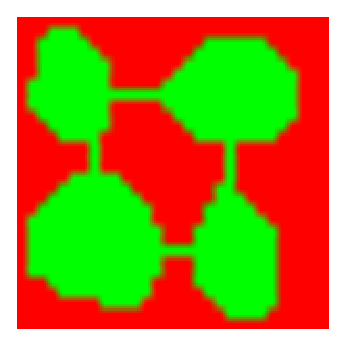
\includegraphics [scale=1]{images/four_caves_map.eps}
  \caption{Map of environment in Experiment1 --- Four Caves.}
  \label{img.four_caves_map}
\end{center}
\end{figure}

\begin{figure}
\begin{center}
  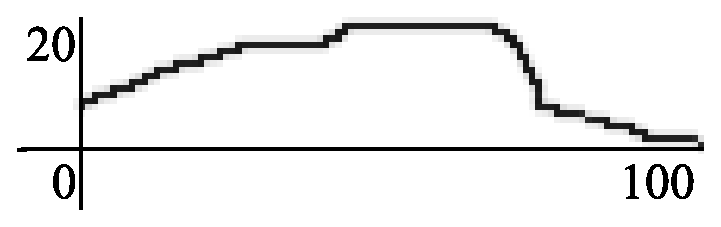
\includegraphics [scale=0.5]{images/four_caves_eff.eps}
  \caption{Course of function Energy From Flower in Experiment1 --- Four Caves. Horizontal vertex = time: 0 .. 100th update, vertical vertex = energy: 0--20.}
  \label{img.four_caves_eff}
\end{center}
\end{figure}

Initial number of beetles is 100, their features were chosen randomly with rule "step on flower" and "noexpectations". The first rule means that all initial beetles decide to make a step when they are hungry and there is a flower in from of them. The second means that feature Expectation on parter is initially set to maximal intervals and thus every two beetles can mate without restrictions of expectations. Costs of actions were set to 2 for a step, 2 for a turn, 3 for mating and 1 for waiting. Mutation rate was 2\%. 30,000 updates were made. The used function of energy from flower (EFF function) is shown in figure \ref{img.four_caves_eff}. The EFF function borders the age of beetles by approximately 100 years.



\begin{figure}
\begin{center}
  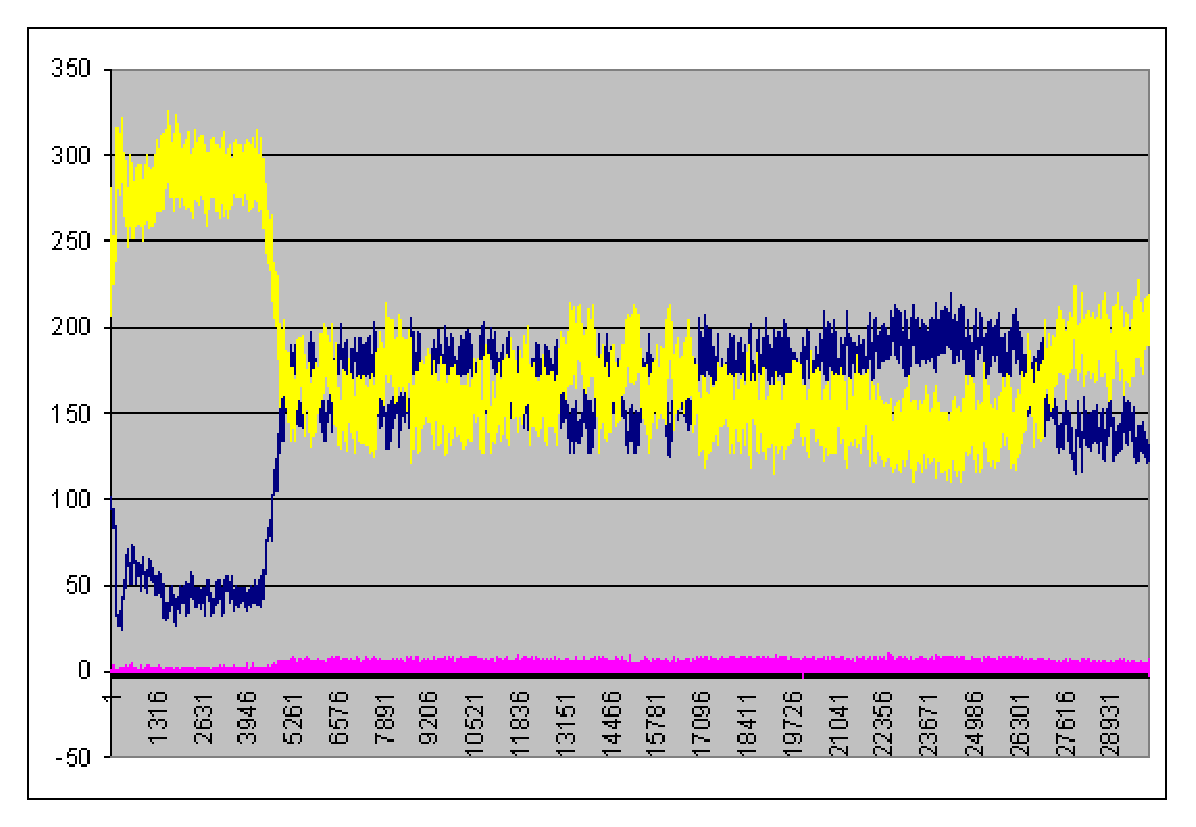
\includegraphics [scale=0.6]{images/Exp1_1_time.eps}
  \caption{Run 1 Experiment1 --- Four Caves.}
  \label{img.four_caves_run1_time}
\end{center}
\end{figure}

\begin{figure}
\begin{center}
  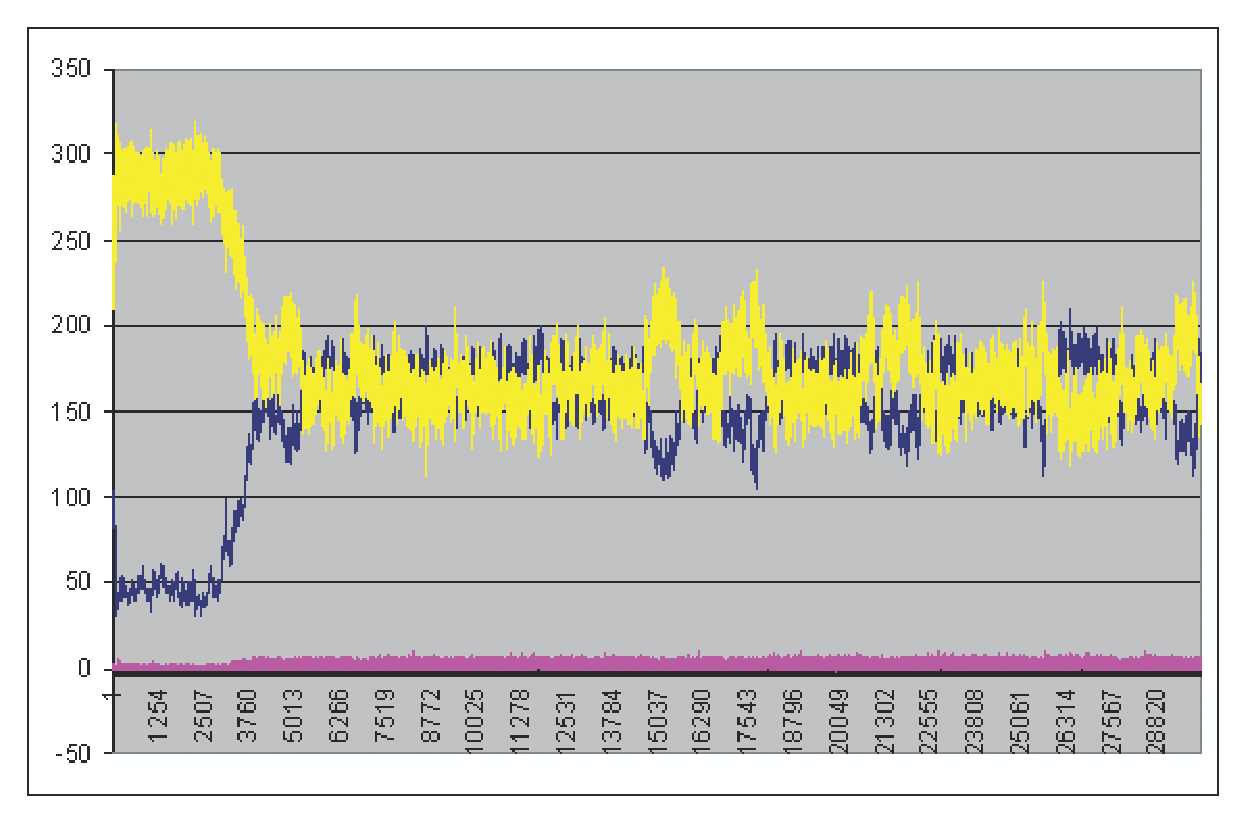
\includegraphics [scale=0.6]{images/Exp1_2_time.eps}
  \caption{Run 2 Experiment1 --- Four Caves.}
  \label{img.four_caves_run2_time}
\end{center}
\end{figure}

\begin{figure}
\begin{center}
  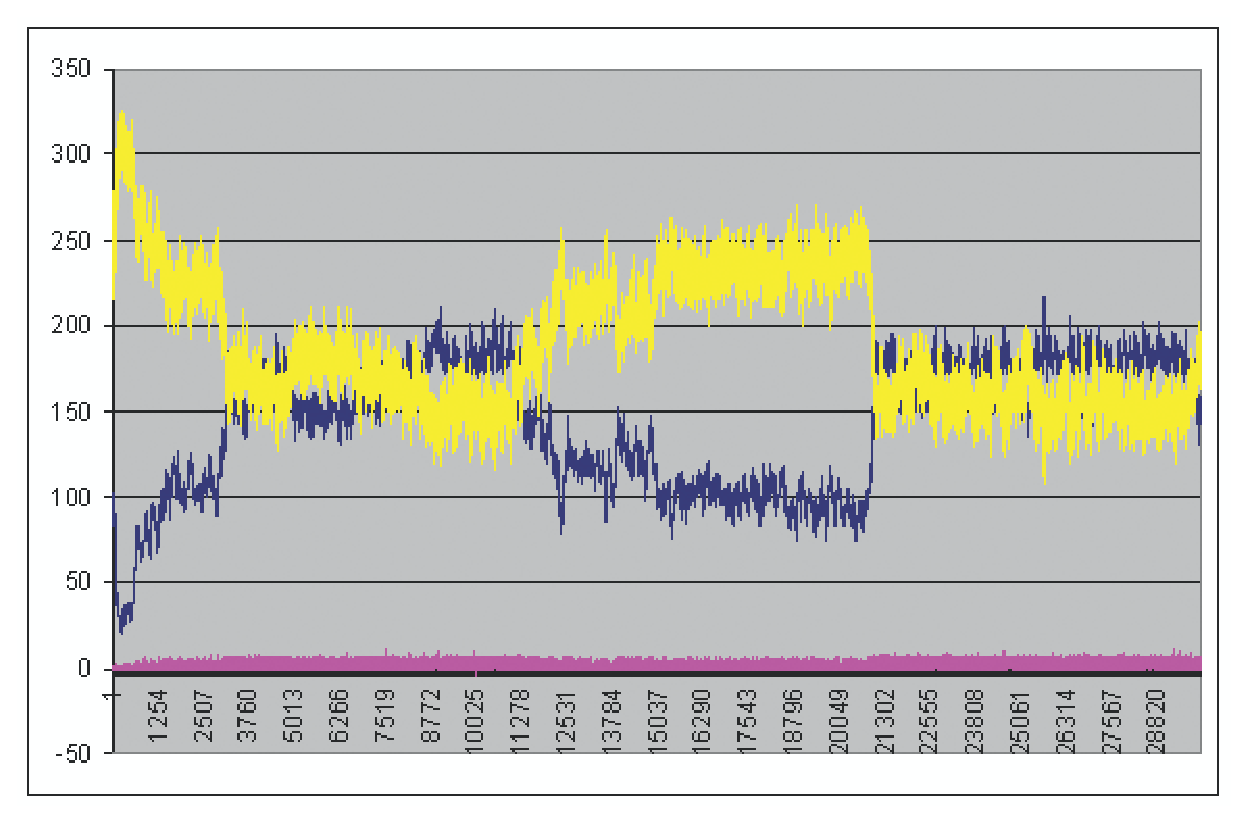
\includegraphics [scale=0.6]{images/Exp1_3_time.eps}
  \caption{Run 3 Experiment1 --- Four Caves.}
  \label{img.four_caves_run3_time}
\end{center}
\end{figure}

\begin{figure}
\begin{center}
  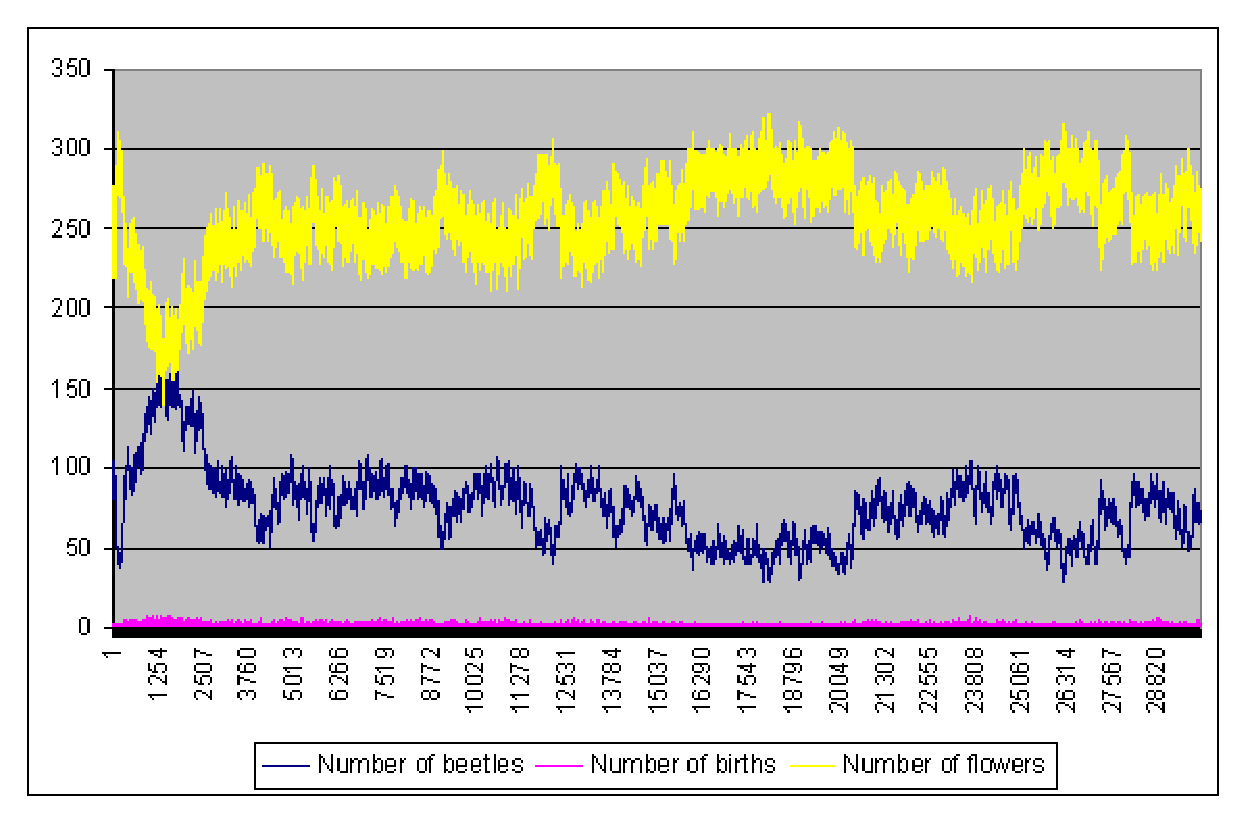
\includegraphics [scale=0.6]{images/Exp1_4_time.eps}
  \caption{Run 4 Experiment1 --- Four Caves.}
  \label{img.four_caves_run4_time}
\end{center}
\end{figure}

The experiment contains four runs with seeds 300, 350, 400 and 450 for generator of pseudorandom numbers. 



\subsection{Results of the Experiment}
%Development of number of beetles in time..extincion and inhabitation of a new cave

Development of population in the four runs of the experiment is in figures \ref{img.four_caves_run1_time}, \ref{img.four_caves_run2_time}, \ref{img.four_caves_run3_time} and \ref{img.four_caves_run4_time}. Number of beetles, number of flowers and number on new born beetles are shown in the figures.
 
Differences among the four graphs of development of populations in the four runs show that coincidence influences the course of runs significantly --- each of them is different.

In all four cases the initial number of beetles falls under half of it at first. This is a general event that happens at the beginning of every simulation with random beetles. A plenty of them are not able to survive, because the random values are not suitable. Only one or two caves remain populated. But children of these beetles are already able to cope with the situation better and they keep the life in the caves. Through corridors they get to neigboring cells and when the number of immigrants is high enough the new cave is inhabited. Inhabitation of a free cave is visible in the graphs, as the number of beetles jumps swiftly by about 50. In run 1 around 4,800th update two empty caves are inhabited, population increased by approximately 100. Between 12,000th and 15,000th update the fourth cave was and was not inhabited alternately. Similarly the development of population in caves can be observed in the other three runs.
 
From the development of population in the experiment can be concluded that beetles with the introduced settings are able to inhabitate empty areas through a narrow corridor. Inhabitation in the scope of Abeetles means that the density of population in the cave is high enough to be independent on immigration from other caves. In other words there are enough beetles to meet, mate and thereby keep the population. On the other hand, if the population shinks under certain size, it becomes extinct in the cave. 

 
\begin{figure}
\begin{center}
  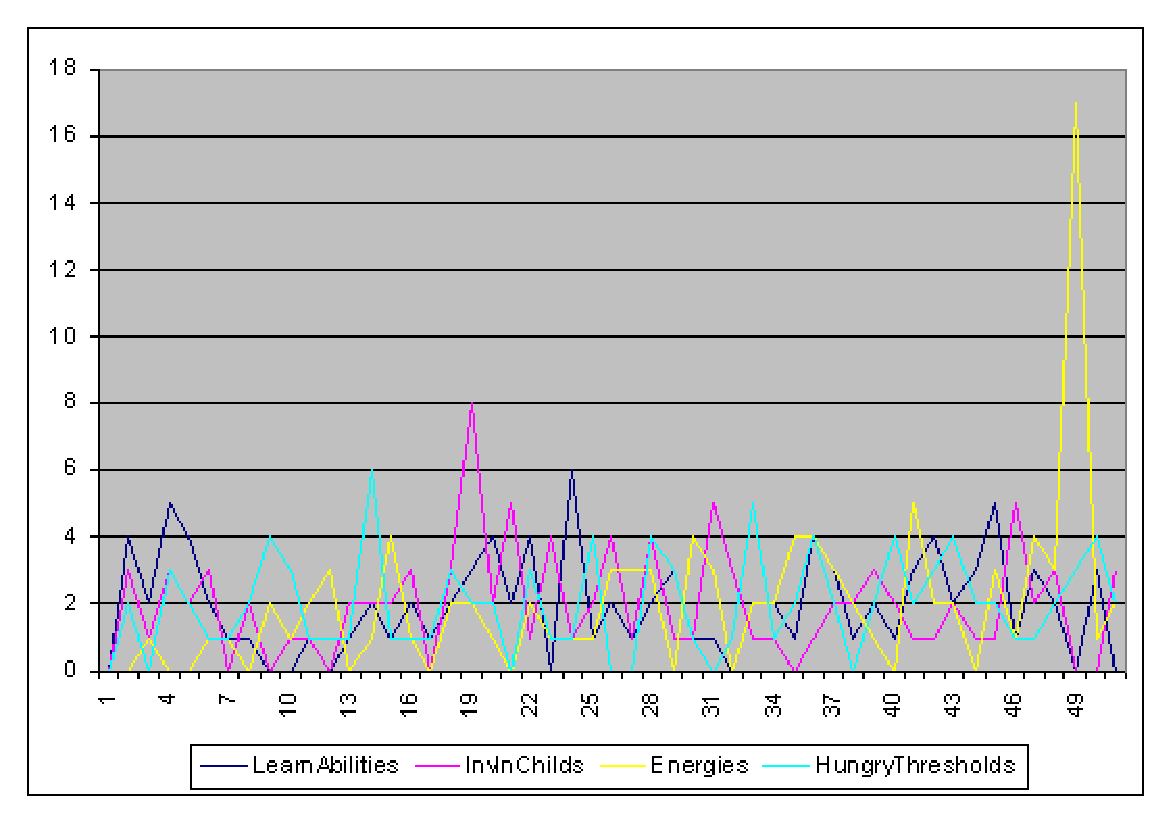
\includegraphics [scale=0.6]{images/Exp1_1_hist0.eps}
  \caption{Run 1 Experiment1 --- Four Caves, histogram of features of beetles at the beginning.}
  \label{img.four_caves_run1_hist0}
\end{center}
\end{figure}

\begin{figure}
\begin{center}
  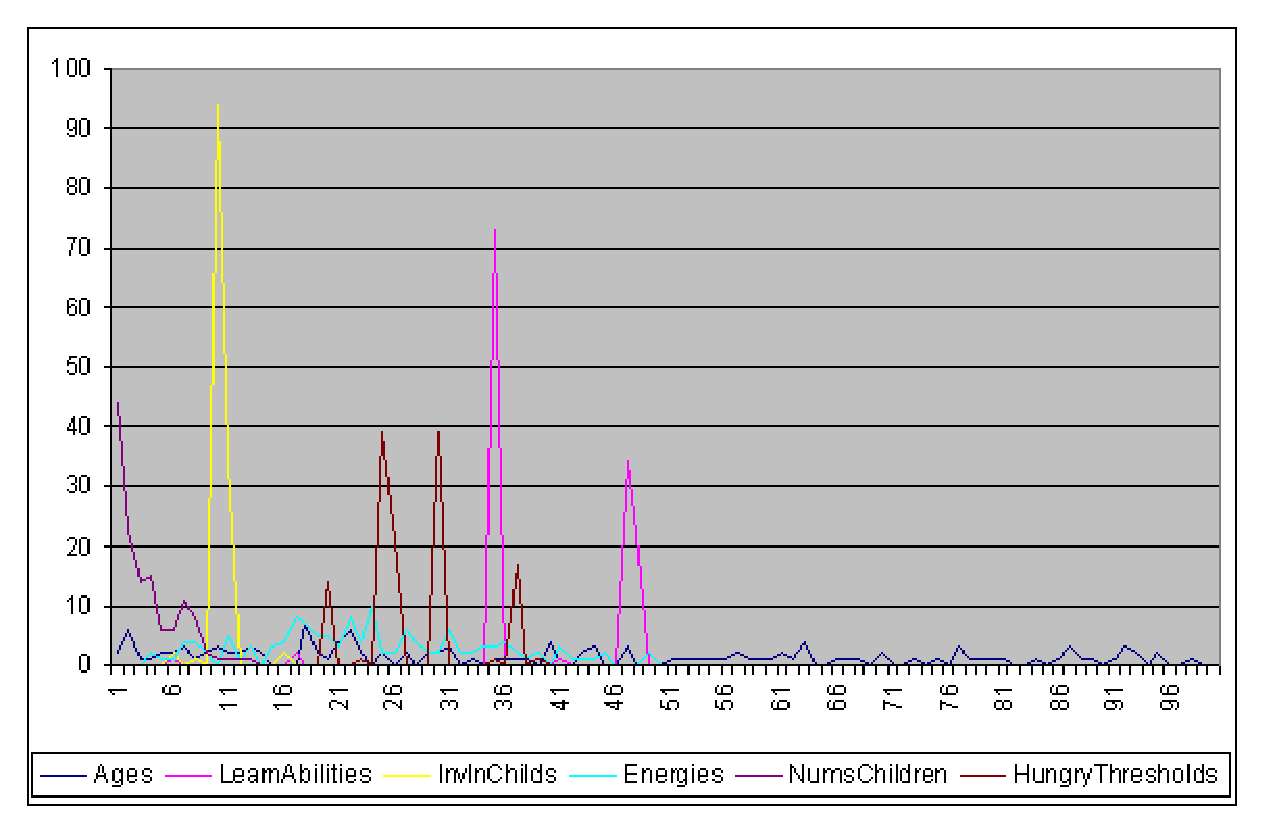
\includegraphics [scale=0.6]{images/Exp1_1_hist30000.eps}
  \caption{Run 1 Experiment1 --- Four Caves, histogram of features of beetles after 30,000th update.}
  \label{img.four_caves_run1_hist30000}
\end{center}
\end{figure}
 
 %Features of beetles.. initial and evolved.
Features of beetles developed interestingly in the experiment. Initial features of beetles were random. So as to support the problematic initial period, expectations on partners were set to maximal intervals. Figure \ref{img.four_caves_run1_hist0} shows the distribution of values of features of beetles at the beginning of run 1 and figure \ref{img.four_caves_run1_hist30000} describes the situation after 30,000 updates. The values of features can be 0 -- 50, only age goes up to 100.

The fluctuation of age is low, no significant death rate of any age group can be observed. Thus the EFF function gives enough chance to survive in any time.
 
Random learn abilities from the beginning narrowed to two major values (35 and 48) and several minor values. In other experiments these values also show direction of development towards several values. In run 2 the major values of learn ability are 4 (133 beetles) and 13 (31 beetles). In run 3 learn abilities narrowed to 4 values and in run 4 to 2 values.
Investment in child also narrowed in run 1, to values 11 and 12. Other runs the results are similar.

The reduction of values of these two features is a general effect of any run of Abeetles. It is a result of the fact that these two features are also subject of expectations on partner. The expectation on a partner's learning ability of a beetle is set as a deviation from the value of learning ability of the beetle. Thus if they both have the same values, they are always suitable partner for the other one no matter what are the expectations. And therefore a group of beetles with similar values can mate more easily. And thanks to this fact and the fact that crossover algorithm with low rate of mutation varies the value only rarely, the particular value from such a group is propagated through children to the next generations more successfully, then from groups of beetles with different values.

There is reciprocial proportion between number of children and number of beetles who have it, which resembles common situation in nature. Hungry thresholds, which are borders between two decision strategies, also narrowed to several values between 20 and 38. This is probably suitable border for this type of map with the 100\% rate of growth of flowers.

\subsection{Subexperiment 1 --- Flowers Die}

If the initial setting of the experiment Four Caves is changed so, that flowers can die with 20\% probability, then they the population becomes extinct rapidly,in run 1 after 440 updates, in run 2 after 1260 updates, in run 3 after 9420 updates, see Figure \ref{img.Exp1_Sub1_3_A_time} and in run 4 after 303 updates. 

When the Subexperiment 1 is run with costs of actions 1,1,2,1, then the population survives in all four cases. It differs from the Experiment 1 in the way that the oscilation range of numbers short slice of time is about 100 whereas in Experiment 1 the oscilation range is about 50. The course of run 2 is in Figure \ref{img.Exp1_Sub1_3_B_time}

\begin{figure}
\begin{center}
  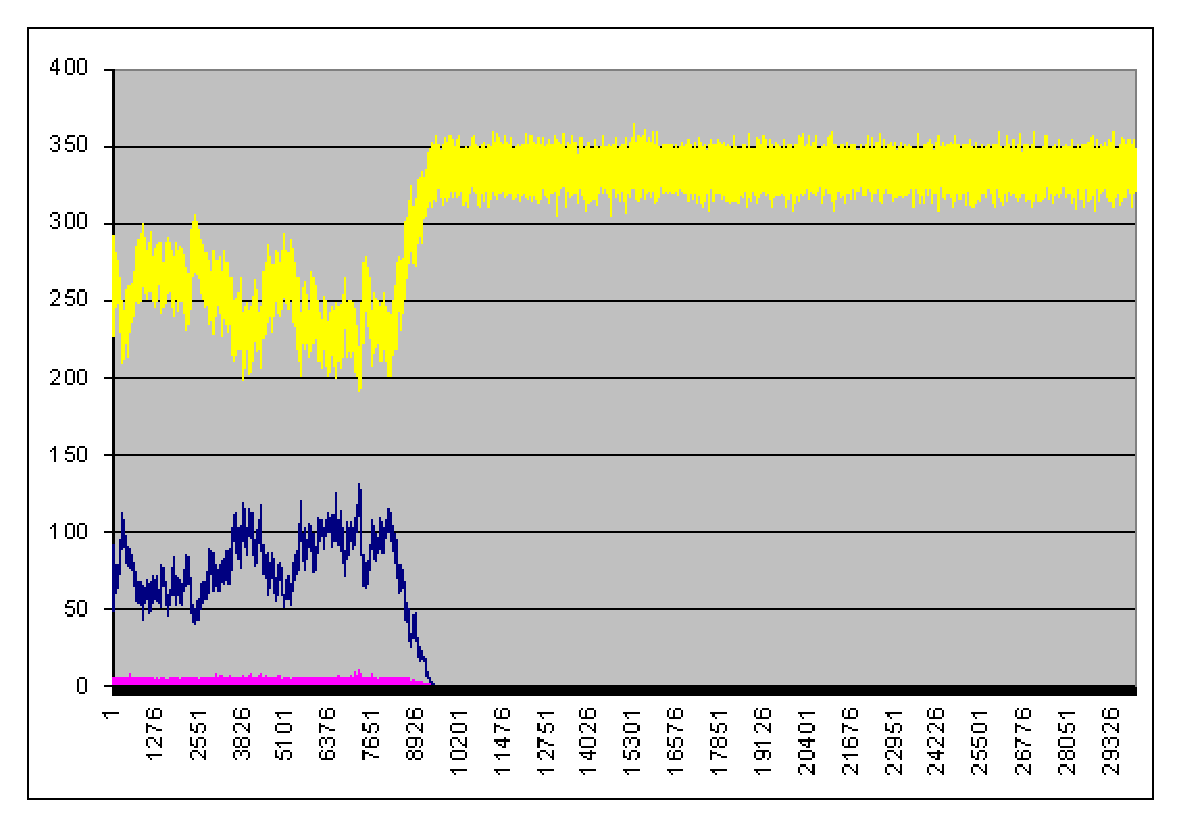
\includegraphics [scale=0.6]{images/Exp1_Sub1_3_A_time.eps}
  \caption{Subexperiment 1 Experiment1 --- Four Caves.}
  \label{img.Exp1_Sub1_3_A_time}
\end{center}
\end{figure}

\begin{figure}
\begin{center}
  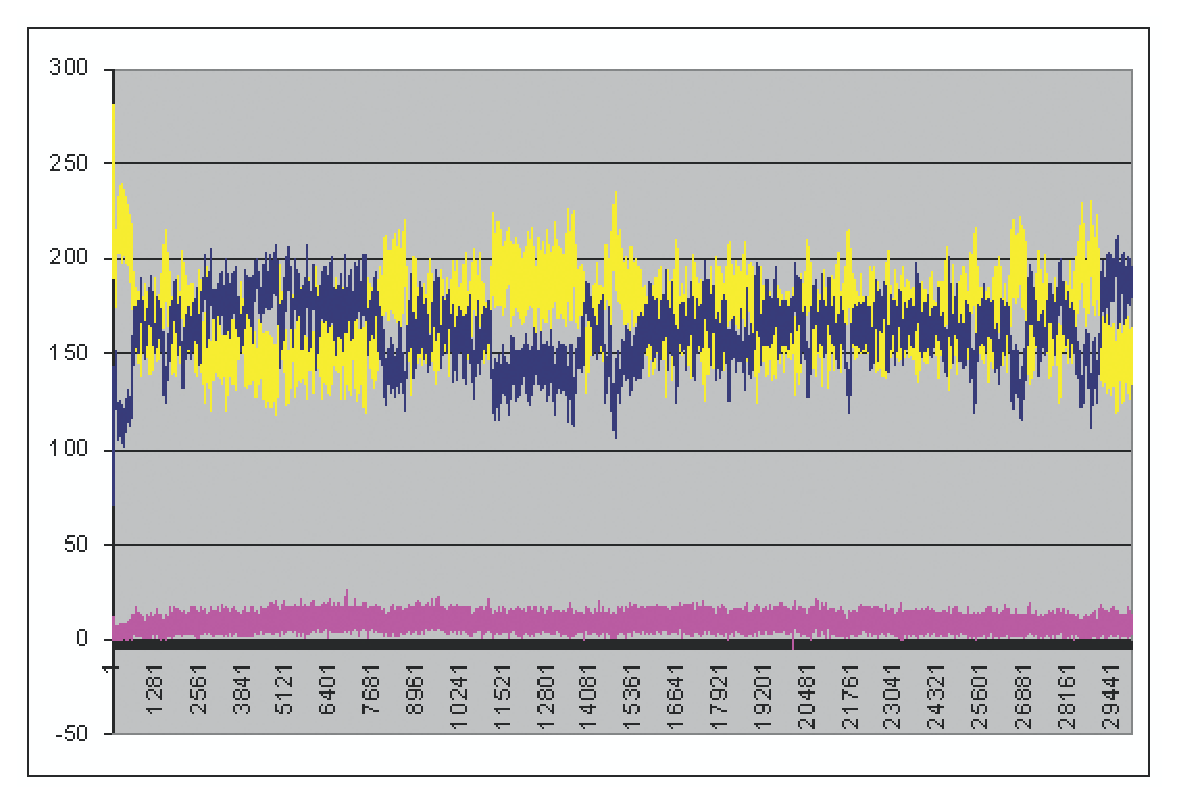
\includegraphics [scale=0.6]{images/Exp1_Sub1_3_B_time.eps}
  \caption{Subexperiment 1 Experiment1 --- Four Caves.}
  \label{img.Exp1_Sub1_3_B_time}
\end{center}
\end{figure}

The subexperiment 1 implies that dying of flowers only decreases the real availability of food for beetles, but does not confuse their ability to survive in more variable environment that changes irregulary.

\subsection{Subexperiment 2 --- Random Initial Expectations}

If the initial expectations are random, the beetles tend much more to become extinct. With 250 beetles at the beginning in all four runs all beetles died within first 320 updates.

\begin{figure}
\begin{center}
  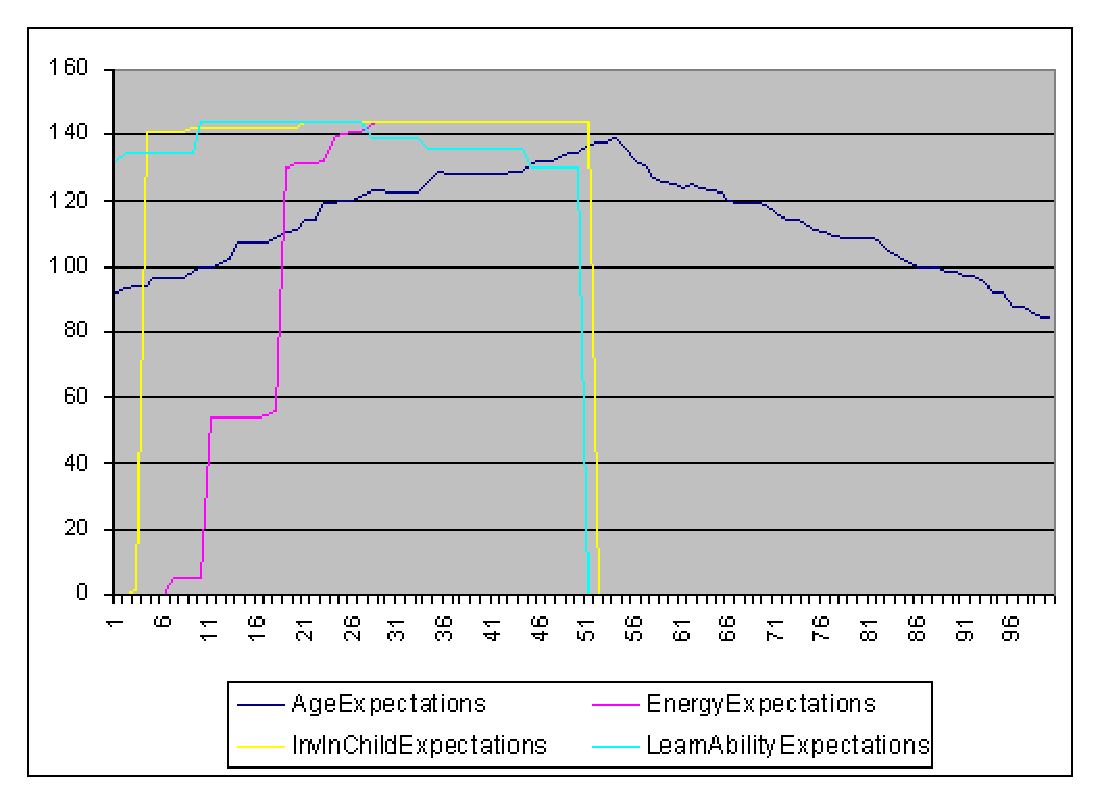
\includegraphics [scale=0.6]{images/Exp1_Sub2_1_histExp.eps}
  \caption{Subexperiment 1 Experiment1 --- Four Caves.}
  \label{img.Exp1_Sub2_1_histExp}
\end{center}
\end{figure}

\begin{figure}
\begin{center}
  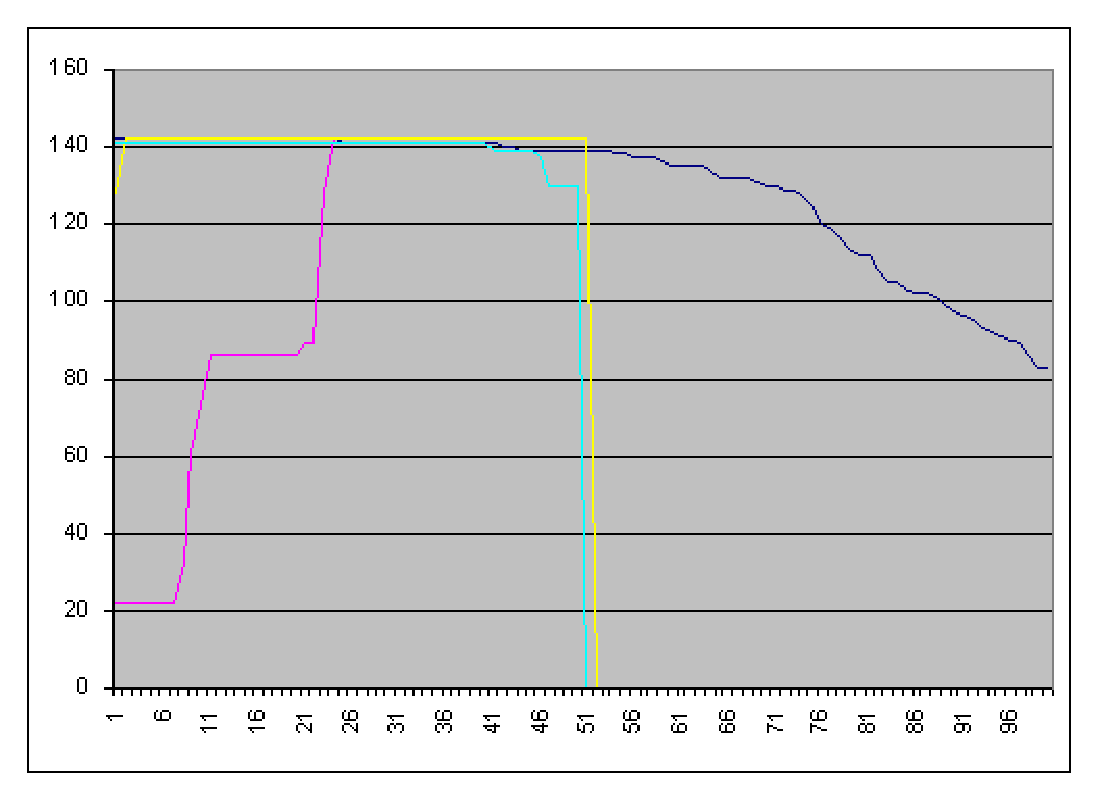
\includegraphics [scale=0.6]{images/Exp1_1_histExp.eps}
  \caption{Run 1 Experiment1 --- histogram after 30,000 updates.}
  \label{img.Exp1_1_histExp}
\end{center}
\end{figure}

Run of this settings was then tried with random seeds and the 16th attempt was successful and population survived all 30,000 updates. At the end there were 144 beetles. Thanks to this success, development of expectation on partner can be observed in the case of random values of expectations. See Figure \ref{img.Exp1_Sub2_1_histExp}. One curve in the histogram, e.g. Age Expectations, shows for how many beetles (axes y) is the value of partners's age (axes x) acceptable.

It can be compared with result of run of Experiment 1 and its histogram after 30,000 updates in \ref{img.Exp1_1_histExp}. It shows that random expectations on a partner allow opportunity for value to vary more, but tendences are not so different from result of case when the ranges of expectations were the widest possible. In that case it is only expectation on energy that changed significantly and can be in connection with the fact that energy at the time of mating is already restricted by hungry threshold. We expected the expectation on investment in child to grow to at least fourth of maximum of energy, but it developed to about 4 (but did not shrink under 2) in case of random initial values and in case of the widest ranges remained 0 for most of beetles but a tenth of them. Even it this case only one beetle in 144 invests less than 2. The result implies that it is enough for a new-born beetle to get 4 pieces of energy at the beginning when costs are 2,2,3,1.

\section{Experiment 2 --- Species of Beetles}

This experiment have for its objective to explore possibilities of development of species of beetles. A species is usually defined as a group of organisms capable of interbreeding and producing fertile offspring. In special case more precise or differing measures are often used, such as based on similarity of DNA or on the presence of specific locally-adapted traits. Nevertheless the precise definition of the term is not clear and discussions about it are referred as the species problem.\cite{Species} 

Species of beetles are defined for the purpose of Abeetles as such groups of beetles that members of one group can never mate with beetles from another group. The difference that would cause such incompatibility can only spring up when expectations and respective features do not match. The group must have at least three members, one or more incompatible beetles often occurs through mutation and die without descendants. Abeetles marks these abnormalities, but they cannot be considered as a real species. 

Species are searched in Abeetles as connected components in an undirected graph. Vertices of the graph are beetles and an edge is between every pair of beetles that have compatible features and expectations on them.
 
The choice of these features is important. A part of expectations concerns energy and age, which cannot be counted as difference between species. Only expectations on investment in children and on learning ability could serve for this purpose. 

\subsection{Initial Settings of the Experiment}
The question is, what initial setting of environment and beetle to choose, so as to reach separation of beetles into species. For separation of species local separation to some extent will be necessary --- beetles should be bred separately. When they are bred totaly separately, it is the same situation as if the two different runs with same general settings is performed and resulting beetles compared. Then species can be bred easily, as it Experiment 1 run 2 values of learning ability are up to 13 and in run 3 at least value 16 is expected. 

Therefore the level of local separation will be searched. First, spaces connected with a corridor of width 1 cell will be examined. For this purpose the map from experiment Four Caves can be used and species can be searched in results of the four runs of that experiment.  

It can be predicted from conclusions of Subexperiment 2 of Experiment 1 that environment of abeetles will not tend to development towards various values of investment in children and expectations on it easily. 

In figure \ref{img.Exp1_Sub2_1_histExp} and figure \ref{img.Exp1_1_histExp} is visible that values of expectations on investment in children have very restricted range and from figure \ref{img.four_caves_run1_hist30000} and other descriptions of results of Experiment 1 is clear that values of investment in children behave similarly.

Development of learning abilities in Experiment 1 was more hopeful, as the values narrowed to two separated ranges, see \ref{img.four_caves_run1_hist30000}. When the situation of the environment is viewed, details of beetles proove that beetles with learning ability 34 live in the bottom left cave and beetles with learning ability 46 live in the bottom right cell (the other two cells are not inhabited). Thus beetles really developed to two different groups, which is for species very promising, even though expectations, see \ref{img.Exp1_1_histExp}, are a wide range over almost all possible values. Therefore this result will be used for this experiment 

In order to it, initial setting of Experiment 2 is the final setting of Experiment 1 run 1. Now various attempts will be done to breed species from these beetles.

\subsection{Results of the Experiment}

The first attempt was to increase mutation rate so as to restrict expectations closer to respective values. The result was that also the value of learning ability started to vary swiftly and also the beetles became extinct in several thousands updates.
 


\begin{figure}
\begin{center}
  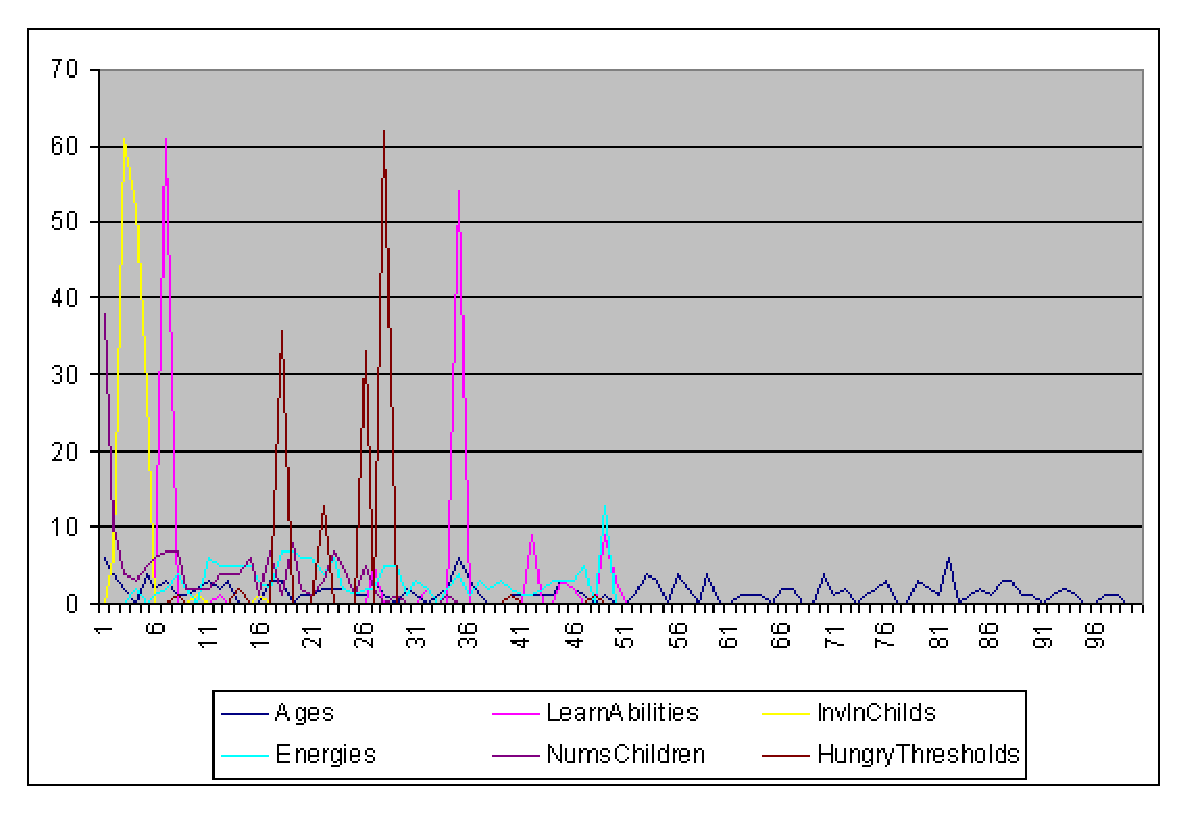
\includegraphics [scale=0.6]{images/Exp1_1_hist365000.eps }
  \caption{Run1 Experiment1 histogram of features of beetles after 365,000 updates.}
  \label{img.Exp1_1_hist365000}
\end{center}
\end{figure}

\begin{figure}
\begin{center}
  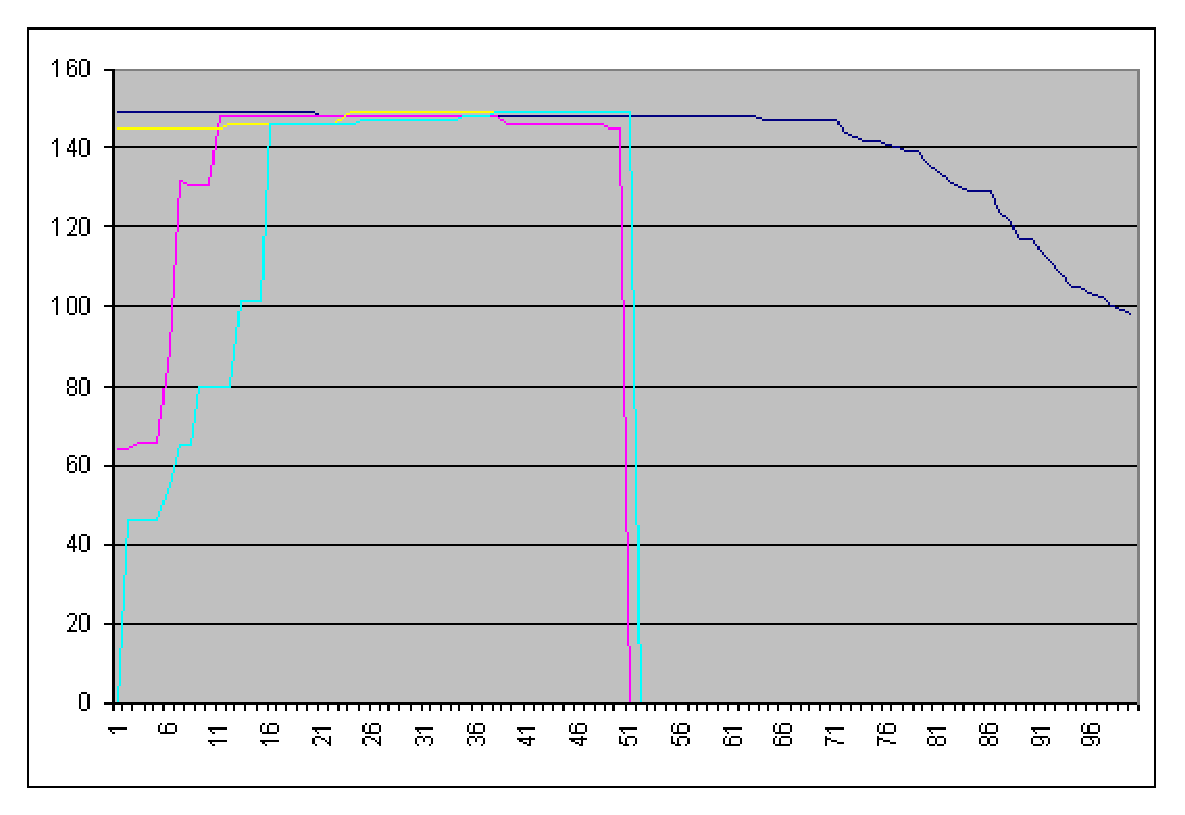
\includegraphics [scale=0.6]{images/Exp1_1_hist365000Exp.eps }
  \caption{Run1 Experiment1 histogram of expectations on partner after 365,000 updates.}
  \label{img.Exp1_1_hist365000Exp}
\end{center}
\end{figure}

\begin{figure}
\begin{center}
  \includegraphics [scale=0.6]{images/Exp2_GUI_species.eps }
  \caption{Run1 Experiment1 histogram of expectations on partner after 365,000 updates.}
  \label{img.Exp2_GUI_species.eps}
\end{center}
\end{figure}
  
The second attempt was to run the environment much longer and leave enough time for evolution to do its work. After roughly 300,000 updates two species of beetles separated, see graphs in figure \ref{img.Exp1_1_hist365000} and figure \ref{img.Exp1_1_hist365000Exp} and situation in \ref{img.Exp2_GUI_species.eps} . But they stayed apart for only about one thousand updates and then beetles from one species passing through corridors prevailed against the other species and the weaker species became extinct. 

To sum up, species in Abeetles can evolve, in separated territories easily, in connected territories it is more difficult and it holds only for a short time.


%%%%%%%%%%%%%%%%%%%%%%%%%%%%%%%%%%%%%%%%%%%%%%%%%%%%%%%%%%%%%%%%%%%%%%%%%%%%%

\chapter{Conclusion}
%Strucne co bylo cilem

Objectives of this thesis were to create simulator Abeetles and run experiments on it. Abeetles focused on five key features. Experiments testing all of them  would be advisable, but scope of the thesis is restricted and therefore only experiments concerning population and species are included.
  
\begin {itemize}
\item Moving strategy --- Abeetles realizes it as a simple decision table and offers only straightforward visualization in a set of tables. It is quite hard to work with it and search for results of evolution. Some better functions that process these results would be contributing. 
\item Learning --- Mutual learning of beetles was realized and offers space for experiments.
\item Choice of partner --- Evolution of choice of partner was important for breeding of species in Abeetles. Realization of expectations as intervals can be considered suitable.
\item Obstacles --- Walls shaping the environment were important for local separation of beetles and searching for species. These objects significanly increases possibilities of experiments.
\item Aging --- Special function for aging was introduced and waits for further experiments. 
\end{itemize}

\noindent Abeetles open possibilities for further searching for interesting results of evolution and offer supporting tools.


\begin{thebibliography}{99}

\bibitem{Bedau}
Mark A. Bedau, 2003, "Artificial life: organization, adaptation and complexity from the bottom up". TRENDS in Cognitive Sciences, \url{http://www.reed.edu/~mab/publications/papers/BedauTICS03.pdf}.

\bibitem{Langton}
Chris G. Langton 1989,  "Artificial Life", Addison-Wesley, \url{http://zooland.alife.org/}.

\bibitem{AdamiBrown}
Chris Adami and Titus Brown, 2000, "What is Artificial Life?" The Seventh International Conference on the Simulation and Synthesis of Living Systems, Reed College, Portland, Oregon, USA.

\bibitem{BornhoffenLataud}
Stefan Bornhofen and Claude Lattaud, 2006, "Artificial Evolution", chapter "Outlines of Artificial Life: A Brief History of Evolutionary Individual Based Models", pages 226--237, Springer.

\bibitem{Delorme}
Marianne Delorme, "An Introduction to Cellular Automata", Cellular Automata: a Parallel Model, Mathematics and Its Application, Kluwer. \url{http://citeseer.ist.psu.edu/delorme98introduction.html}. 

\bibitem{GeneDic}
Gene. (n.d.). Columbia Electronic Encyclopedia. Retrieved from Reference.com website: \url{http://www.reference.com/browse/columbia/gene-ent}.

\bibitem{GenPhen}
Richard Lewontin, "The Genotype/Phenotype Distinction", The Stanford Encyclopedia of Philosophy (Spring 2007 Edition), Edward N. Zalta (ed.), \url{http://plato.stanford.edu/archives/spr2007/entries/genotype-phenotype/}.

\bibitem{GenomeDef}
Joshua Lederberg and Alexa T. McCray, 2001, "'Ome Sweet 'Omics -- A Genealogical Treasury of Words", The Scientist 15 (7), \url{http://lhncbc.nlm.nih.gov/lhc/docs/published/2001/pub2001047.pdf}

\bibitem{Avida}
C. Ofria and C.O. Wilke, 2004, "Avida: A Software Platform for Research in Computational Evolutionary Biology", Artificial Life 10, pages 191--229.

\bibitem{Tierra}
T. S. Ray 1991, "Evolution and optimization of digital organisms", in Billingsley K.R. et al (eds), Scientific Excellence in Supercomputing: The IBM 1990 Contest Prize Papers, Athens, GA, 30602: The Baldwin Press, The University of Georgia, pages 489--531.

\bibitem{GenePool1}
Jeffrey Ventrella, 1998, "Attractiveness vs. Efficiency: How Mate Preference Affects Locomotion in the Evolution of Artificial Swimming Organisms", Artificial Life VI 1998, MIT Press, \url{http://www.ventrella.com/Alife/Attractiveness/attractiveness_0.html}.
 
\bibitem{GenePool2}
Jeffrey Ventrella, 2005, "Gene Pool: Exploring the Interaction Between Natural Selection and Sexual Selection", Chapter 4 in Artificial Life Models in Software, edited by Andrew Adamatzky and Maciej Komosinski, Springer.

\bibitem{Mitozoos}
Bestiario company, "The book of the mitozoos", \url{http://bestiario.org/mitozoos/english/pdf/mitozoos\_en.pdf}. 

\bibitem{Broucci}
Tom\'{a}\v{s} Holan, 2004, Jiné programování "The Different Programming" In Vojt\'{a}\v{s}, Peter, ITAT 2004 Information Technologies – Applications and Theory, Košice: UPJŠ, 2004, pages 139--148, \url{http://ksvi.mff.cuni.cz/~holan/jinak/itat.pdf}

\bibitem{SelfishGene}
Richard Dawkins, The Selfish Gene, 11. Memes:the new replicators, Oxford University, second edition, December 1989, ISBN 0-19-217773-7.

\bibitem{Species}
G. C. Robson, 1928, "The Species Problem: an Introduction to the Study of Evolutionary Divergence in Natural Populations", Oliver and Boyd, Edinburgh.

%\bibitem{PVM versus MPI}
%PVM and MPI: a Comparison of Features; G.A.Geist J.A.Kohl P.M. Papadopoulos

\end{thebibliography}

\end{document}

%cau
%takhle preklada cesky zdroj Vaclav Klimes

% \bibitem{tectogramtic_annotation} Marie Mikulová, ... , Zdeněk Žabokrtský. Anotace Prazžského závislostního korpusu na tektogramatické rovině: pokyny pro anotátory [A Manual for Tectogrammatical Layer Annotation of the Prague Dependency Treebank]. Technical report, ÚFAL, MFF UK, Prague, Czech Republic, 2005. URL http://ufal.mf\/f.cuni.cz/pdt2.0/doc/manuals/cz/t-layer/pdf/t-man-cz.pdf.
